\def\year{2020}\relax
%File: formatting-instruction.tex
\documentclass[letterpaper]{article} % DO NOT CHANGE THIS
\usepackage{aaai20}  % DO NOT CHANGE THIS
\usepackage{times}  % DO NOT CHANGE THIS
\usepackage{helvet} % DO NOT CHANGE THIS
\usepackage{courier}  % DO NOT CHANGE THIS
\usepackage[hyphens]{url}  % DO NOT CHANGE THIS
\usepackage{graphicx} % DO NOT CHANGE THIS
\urlstyle{rm} % DO NOT CHANGE THIS
\def\UrlFont{\rm}  % DO NOT CHANGE THIS
\usepackage{graphicx}  % DO NOT CHANGE THIS
\frenchspacing  % DO NOT CHANGE THIS
\setlength{\pdfpagewidth}{8.5in}  % DO NOT CHANGE THIS
\setlength{\pdfpageheight}{11in}  % DO NOT CHANGE THIS
%\nocopyright
%PDF Info Is REQUIRED.
% For /Author, add all authors within the parentheses, separated by commas. No accents or commands.
% For /Title, add Title in Mixed Case. No accents or commands. Retain the parentheses.
 % \pdfinfo{
% /Title (AAAI Press Formatting Instructions for Authors Using LaTeX -- A Guide)
% /Author (AAAI Press Staff, Pater Patel Schneider, Sunil Issar, J. Scott Penberthy, George Ferguson, Hans Guesgen)
% } %Leave this	
% /Title ()
% Put your actual complete title (no codes, scripts, shortcuts, or LaTeX commands) within the parentheses in mixed case
% Leave the space between \Title and the beginning parenthesis alone
% /Author ()
% Put your actual complete list of authors (no codes, scripts, shortcuts, or LaTeX commands) within the parentheses in mixed case. 
% Each author should be only by a comma. If the name contains accents, remove them. If there are any LaTeX commands, 
% remove them. 

%%%%%%%%%%%%%%%%%%%%%%%%%%%%%%%%%%%
% customized packages and commands
\usepackage{url}
\usepackage{subfigure}
\usepackage{amsmath}
\usepackage{amssymb}
\usepackage{xcolor}
\newcommand{\overbar}[1]{\mkern 1.5mu\overline{\mkern-1.5mu#1\mkern-1.5mu}\mkern 1.5mu}
% \usepackage[noend]{algpseudocode}
\usepackage{algorithm}
\usepackage[noend]{algorithmic}
\newcommand{\red}[1]{\textcolor{red}{#1}}
\newcommand{\blue}[1]{\textcolor{blue}{#1}}
\newcommand{\bs}[1]{\boldsymbol{#1}}
\newtheorem{defi}{Definition}
\newtheorem{lemma}{Lemma}
\newtheorem{theorem}{Theorem}
\newtheorem{assume}{Assumption}
\newtheorem{coro}{Corollary}

\usepackage{mdframed}
\usepackage{lipsum}
\newmdtheoremenv{algo}{Algorithm}

% for algorithm indentation
\newlength\myindent
\setlength\myindent{1.5em}
\newcommand\bindent{%
  \begingroup
  \setlength{\itemindent}{\myindent}
  \addtolength{\algorithmicindent}{\myindent}
}
\newcommand\eindent{\endgroup}
%%%%%%%%%%%%%%%%%%%%%%%%%%%%%%%%%%%

% DISALLOWED PACKAGES
% \usepackage{authblk} -- This package is specifically forbidden
% \usepackage{balance} -- This package is specifically forbidden
% \usepackage{caption} -- This package is specifically forbidden
% \usepackage{color (if used in text)
% \usepackage{CJK} -- This package is specifically forbidden
% \usepackage{float} -- This package is specifically forbidden
% \usepackage{flushend} -- This package is specifically forbidden
% \usepackage{fontenc} -- This package is specifically forbidden
% \usepackage{fullpage} -- This package is specifically forbidden
% \usepackage{geometry} -- This package is specifically forbidden
% \usepackage{grffile} -- This package is specifically forbidden
% \usepackage{hyperref} -- This package is specifically forbidden
% \usepackage{navigator} -- This package is specifically forbidden
% (or any other package that embeds links such as navigator or hyperref)
% \indentfirst} -- This package is specifically forbidden
% \layout} -- This package is specifically forbidden
% \multicol} -- This package is specifically forbidden
% \nameref} -- This package is specifically forbidden
% \natbib} -- This package is specifically forbidden -- use the following workaround:
% \usepackage{savetrees} -- This package is specifically forbidden
% \usepackage{setspace} -- This package is specifically forbidden
% \usepackage{stfloats} -- This package is specifically forbidden
% \usepackage{tabu} -- This package is specifically forbidden
% \usepackage{titlesec} -- This package is specifically forbidden
% \usepackage{tocbibind} -- This package is specifically forbidden
% \usepackage{ulem} -- This package is specifically forbidden
% \usepackage{wrapfig} -- This package is specifically forbidden
% DISALLOWED COMMANDS
% \nocopyright -- Your paper will not be published if you use this command
% \addtolength -- This command may not be used
% \balance -- This command may not be used
% \baselinestretch -- Your paper will not be published if you use this command
% \clearpage -- No page breaks of any kind may be used for the final version of your paper
% \columnsep -- This command may not be used
% \newpage -- No page breaks of any kind may be used for the final version of your paper
% \pagebreak -- No page breaks of any kind may be used for the final version of your paperr
% \pagestyle -- This command may not be used
% \tiny -- This is not an acceptable font size.
% \vspace{- -- No negative value may be used in proximity of a caption, figure, table, section, subsection, subsubsection, or reference
% \vskip{- -- No negative value may be used to alter spacing above or below a caption, figure, table, section, subsection, subsubsection, or reference

\setcounter{secnumdepth}{2} %May be changed to 1 or 2 if section numbers are desired.

% The file aaai20.sty is the style file for AAAI Press 
% proceedings, working notes, and technical reports.
%
\setlength\titlebox{2.5in} % If your paper contains an overfull \vbox too high warning at the beginning of the document, use this
% command to correct it. You may not alter the value below 2.5 in
\title{Learning Privately over Distributed Features:\\An ADMM Sharing Approach}
%Your title must be in mixed case, not sentence case. 
% That means all verbs (including short verbs like be, is, using,and go), 
% nouns, adverbs, adjectives should be capitalized, including both words in hyphenated terms, while
% articles, conjunctions, and prepositions are lower case unless they
% directly follow a colon or long dash
% \author{Written by AAAI Press Staff\textsuperscript{\rm 1}\thanks{Primarily Mike Hamilton of the Live Oak Press, LLC, with help from the AAAI Publications Committee}\\ \Large \textbf{AAAI Style Contributions by
% Pater Patel Schneider,} \\ \Large \textbf{Sunil Issar, J. Scott Penberthy, George Ferguson, Hans Guesgen}\\ % All authors must be in the same font size and format. Use \Large and \textbf to achieve this result when breaking a line
% \textsuperscript{\rm 1}Association for the Advancement of Artificial Intelligence\\ %If you have multiple authors and multiple affiliations
% use superscripts in text and roman font to identify them. For example, Sunil Issar,\textsuperscript{\rm 2} J. Scott Penberthy\textsuperscript{\rm 3} George Ferguson,\textsuperscript{\rm 4} Hans Guesgen\textsuperscript{\rm 5}. Note that the comma should be placed BEFORE the superscript for optimum readability
% 2275 East Bayshore Road, Suite 160\\
% Palo Alto, California 94303\\
% publications20@aaai.org % email address must be in roman text type, not monospace or sans serif
% }
\begin{document}

\maketitle

\begin{abstract}
Distributed machine learning has been widely studied in order to handle exploding amount of data.
In this paper, we study an important yet less visited distributed learning problem where features are inherently distributed or vertically partitioned among multiple parties, and sharing of raw data or model parameters among parties is prohibited due to privacy concerns.
We propose an ADMM sharing framework to approach risk minimization over distributed features, where each party only needs to share a single value for each sample in the training process, thus minimizing the data leakage risk.
%workshop change
% \emph{We establish convergence and iteration complexity results for the proposed parallel ADMM algorithm under non-convex loss. We further introduce a novel differentially private ADMM sharing algorithm and bound the privacy guarantee with carefully designed noise perturbation. The experiments based on a prototype system shows that the proposed ADMM algorithms converge efficiently in a robust fashion, demonstrating advantage over gradient based methods especially for data set with high dimensional feature spaces.}
We introduce a novel differentially private ADMM sharing algorithm and bound the privacy guarantee with carefully designed noise perturbation. The experiments based on a prototype system shows that the proposed ADMM algorithms converge efficiently in a robust fashion, demonstrating advantage over gradient based methods especially for data set with high dimensional feature spaces.
\end{abstract}

\section{Introduction}
\red{Introductory examples from hospital, bank, government, etc.}

Distributed machine learning has been widely studied in order to handle exploding amount of data. It has also been reported that the volume and quality of data determines the upper bound of machine learning model performance. Privacy-preserving technique in distributed machine learning is one of the keys to encourage data sharing in distributed system. There are mainly two lines of works in privacy-preserving, encryption and differential privacy. Although encryption based methods have strong guarantee for data security, it has heavy computation overhead, which is not scalable. Differential privacy (DP) based methods are light weighted. Well designed DP algorithm can achieve good model performance under certain privacy guarantee. 

Most existing DP distributed machine learning works focus on data parallel scenario, where different subsets of the samples are distributed. To the best of our knowledge, few works are on the model parallel scenario, where different subset of the features are distributed. 

% \begin{figure}[t]
%     \centering
%     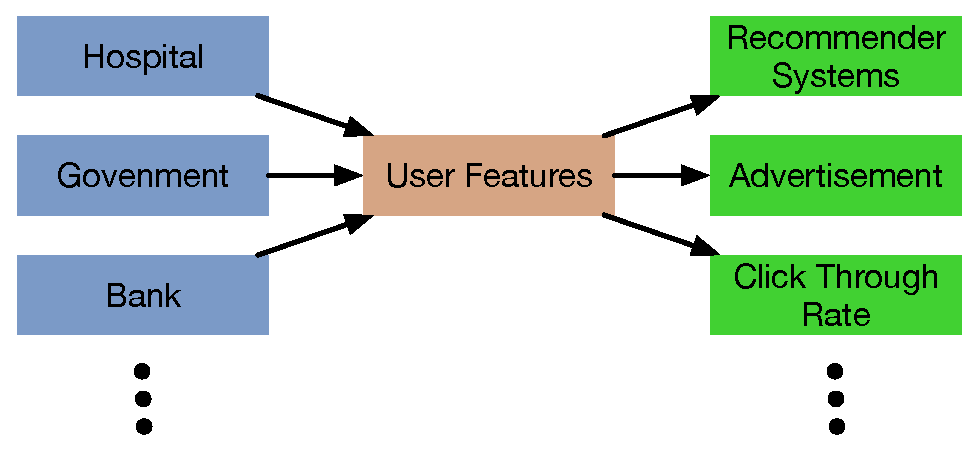
\includegraphics[width=3.2in]{figures/application.eps}
%     \caption{Applying Sensitive User Features to Other Applications}
%     \label{fig:application}
%     \vspace{-5mm}
% \end{figure}

We propose an efficient solution for the real application where features are distributed. In distributed machine learning system, convergence is a comprehension results of computation and communication. \red{In the case, ADMM sharing is a best suit since it is fast to converge in terms of epochs, which requires less privacy budget given certain accuracy.}


\section{Machine Learning over Distributed Features}
Consider feature data for $N$ samples are distributed on $m$ parties. On each party $j$, $D^j\in\mathbb{R}^N\times\mathbb{R}^{d_j}$ is the feature dataset where $d_j$ is the feature dimension on party $j$ and we denote $d=\sum_id_i$ the total feature dimension. We denote the $i^{th}$ row of $D_j$ as $D_j^i$. We denote the concatenated features as $D$. $Y\in\{-1, 1\}^N$ is the label for the samples with $Y^i$ denoting the $i^{th}$ label. $(D_1, D_2, \ldots, D_m, Y)$ is the total training data. We need to find a model $f(D_1^i, D_2^i, \ldots, D_m^i, x)$ with parameters $x$ to predict the labels that minimizes some predefined loss $l(f, Y)$ between the predicted labels and the true labels. 
\begin{align}
\underset{x}{\text{minimize}}&\quad\frac{1}{N}\sum_i l_i(f(D_1^i, D_2^i, \ldots, D_m^i; x), Y^i) + \lambda R(x), \label{eq:ori_problem}\\
\text{s.t.}&\quad x \in X,
\end{align}
where $X\subset\mathbb{R}^d$ is a closed convex set; $R(\cdot)$ is some regularizor; $\lambda$ is some tunable coefficient. 
% We consider \emph{generalized additive models}
We consider models that linearly depends on the features
% \begin{align}
% f(D_1^i, D_2^i, \ldots, D_m^i, x) = \sigma(\sum_j h_j(D_j^i, x_j)),
% \end{align}
\begin{align}
f(D_1^i, D_2^i, \ldots, D_m^i, x) = \sigma(\sum_j D_j^i, x_j),
\end{align}
% where $h_j(\cdot, \cdot)$ is some local aggregation function for the features on party $j$
where $\sigma(\cdot)$ is some activation function. This class of functions include a wide range of realistic models such as lasso, logistic regression, SVM, etc. 
Taking logistic regress as example, we have
\begin{align}
f(D_1^i, D_2^i, \ldots, D_m^i, x) = 1/(1+\text{exp}(-\sum_j D_j^ix_j)),
\end{align}
and 
\begin{align}
l_i(f^i, Y^i) = & 1/(1+\text{exp}(-Y^i\sum_j D_j^ix_j)).
\end{align}

Considering separable regularizor where
\begin{align}
R(x) = \sum_j R_j(x_j),
\end{align}
and rewriting it in a more compact format, the problem is 
\begin{align}
\underset{x}{\text{minimize}}&\quad l\left(\sum_j D_jx_j\right) + \lambda\sum_j R_j(x_j), \label{eq:analysis_problem}\\
\text{s.t.}&\quad x_j\in X_j, j=1,\ldots,m,
\end{align}
where  $X_j\subset\mathbb{R}^{d_j}, \forall j$ are closed convex sets. 


\section{The ADMM Sharing Algorithm}
\label{sec:admmSharing}
We present an ADMM sharing algorithm \cite{boyd2011distributed,hong2016convergence} to solve Problem~\eqref{eq:analysis_problem} \emph{and establish a convergence guarantee for the algorithm.} Our algorithm requires each party only share a single value to other parties in each iteration, thus requiring the minimum message passing. 
In particular, Problem~\eqref{eq:analysis_problem} is equivalent to
\begin{align}
\underset{x}{\text{minimize}} &\quad l\left(z\right) + \lambda\sum_{m=1}^{M} R_m(x_m),\\
\text{s.t.} &\quad \sum_{m=1}^{M} \mathcal{D}_m x_m - z = 0,\quad x_m\in X_M, m=1,\ldots,M,
\end{align}
where $z$ is an auxiliary variable. 
% Define $\{x\}=\{x_1,\cdots,x_M\}$.
The corresponding augmented Lagrangian is given by
\begin{align}
\mathcal{L}(\{x\}, z; y) =& l(z) + \lambda\sum_{m=1}^{M} R_m(x_m) + \langle y, \sum_{m=1}^{M}\mathcal{D}_m x_m - z\rangle \nonumber\\
    &+ \frac{\rho}{2}\|\sum_{m=1}^{M} \mathcal{D}_m x_m - z\|^2, \label{eq:lagragian}
\end{align}
where $y$ is the dual variable and $\rho$ is the penalty factor.
In the $t^{th}$ iteration of the algorithm, variables are updated according to
% {\bf the sequential updating algorithm}
% \begin{align}
% &x_j^{t+1}:=\underset{x_j\in X_j}{\text{argmin}}\quad\lambda R_j(x_j) + \langle y^t, D_jx_j\rangle + \frac{\rho}{2}\big\|\sum_{k<j}D_kx_k^{t+1} + \sum_{k>j}D_kx_k^t + D_jx_j - z^t\big\|^2\label{eq:seq_algo_x}\\
% &z^{t+1}:=\underset{z}{\text{argmin}}\quad l(z) - \langle y^t, z \rangle + \frac{\rho}{2} \big\|\sum_jD_jx_j^{t+1} - z\big\|^2\label{eq:seq_algo_z}\\
% &y^{t+1}:=y^t + \rho\big(\sum_jD_jx_j^{t+1} - z^{t+1}\big),\label{eq:seq_algo_y}
% \end{align}
% and  {\bf the parallel updating algorithm}

\begin{align}
&x_m^{t+1}:=\underset{x_m\in X_m}{\text{argmin}}\quad\lambda R_m(x_m) + \langle y^t, \mathcal{D}_mx_m\rangle\nonumber\\
& \quad\quad\quad\quad\quad\quad\quad+ \frac{\rho}{2}\big\|\sum_{\substack{k=1,~k\neq m}}^{M}\mathcal{D}_kx_k^{t} + \mathcal{D}_mx_m - z^t\big\|^2, \nonumber\\
&\hspace*{36pt} m=1,\cdots,M\label{eq:pal_algo_x}\\
&z^{t+1}:=\underset{z}{\text{argmin}}\quad l(z)  - \langle y^t, z \rangle + \frac{\rho}{2} \big\|\sum_{m=1}^{M}\mathcal{D}_mx_m^{t+1} - z\big\|^2\label{eq:pal_algo_z}\\
&y^{t+1}:=y^t + \rho\big(\sum_{m=1}^{M}\mathcal{D}_mx_m^{t+1} - z^{t+1}\big).\label{eq:pal_algo_y}
\end{align}

Formally, in a distributed and fully parallel manner, the algorithm is described in Algorithm~\ref{alg:ADMM_sharing}. Note that each party $m$ needs the value $\sum_{k\neq m}\mathcal{D}_kx_k^{t} - z^{t}$ to complete the update, and Lines~\ref{alg:line_1}, \ref{alg:line_2} and \ref{alg:line_8} in Algorithm~\ref{alg:ADMM_sharing} present a trick to reduce communication overhead. On each local party , \eqref{eq:pal_algo_x} is computed where a proper $x_m$ is derived to simultaneously minimize the regularizer and bring the global prediction close to $z^t$, given the local predictions from other parties. When $R_m(\cdot)$ is $l_2$ norm, \eqref{eq:pal_algo_x} becomes a trivial quadratic program which can be efficiently solved. On the central node, the global prediction $z$ is found in \eqref{eq:pal_algo_z} by minimizing the loss $l(\cdot)$ while bringing $z$ close to the aggregated local predictions from all local parties. Therefore, the computational complexity of \eqref{eq:pal_algo_z} is independent of the number of features, thus making the proposed algorithm scalable to a large number of features, as compared to SGD or Frank-Wolfe algorithms. %The central node updates $y$ by \eqref{eq:pal_algo_y} after it updates $z$.

\begin{algorithm}[t]
\caption{The ADMM Sharing Algorithm}
\begin{algorithmic}[1]
    \STATE -----\emph{Each party $m$ performs in parallel:}
    % \bindent
    \FOR {$t$ in $1, \ldots, T$}
        \STATE Pull  $\sum_k\mathcal{D}_kx_k^{t} - z^{t}$  and $y^{t}$ from central node \label{alg:line_1}
        \STATE Obtain $\sum_{k\neq m}\mathcal{D}_kx_k^{t} - z^{t}$ by subtracting the locally cached $\mathcal{D}_mx_m^{t}$ from  the pulled value $\sum_k\mathcal{D}_kx_k^{t} - z^{t}$ \label{alg:line_2}
        \STATE Compute $x_m^{t+1}$ according to \eqref{eq:pal_algo_x} \label{alg:line_3}
        \STATE Push $\mathcal{D}_mx_m^{t+1}$ to the central node \label{alg:line_4}
    \ENDFOR
    % \eindent
    \STATE -----\emph{Central node:}
    % \bindent
    \FOR{$t$ in $1, \ldots, T$}
        \STATE Collect $\mathcal{D}_mx_m^{t+1}$ for all $m=1,\ldots,M$\label{alg:line_5}
        \STATE Compute $z^{t+1}$ according to \eqref{eq:pal_algo_z}\label{alg:line_6}
        \STATE Compute $y^{t+1}$ according to \eqref{eq:pal_algo_y}\label{alg:line_7}
        \STATE Distribute $\sum_k\mathcal{D}_kx_k^{t+1} - z^{t+1}$  and $y^{t+1}$ to all the parties. \label{alg:line_8}
    \ENDFOR
    % \eindent
\end{algorithmic}
\label{alg:ADMM_sharing}
\end{algorithm}

% \subsection{Privacy Concern and Differential Privacy}

% Random noise added to the query. Variance is correlated to the DP guarantee.
% {\bf Laplace Mechanism}
% \begin{align}
% \eta\sim\text{Lap}(\frac{\Delta f}{\epsilon})
% \end{align}

% ADMM sharing with differential privacy.
% \begin{align}
% &x_m^{t+1}:=\underset{x_m\in X_m}{\text{argmin}}\quad\lambda R_m(x_m) + \langle y^t, \mathcal{D}_mx_m\rangle + \frac{\rho}{2}\big\|\sum_{\substack{k=1\\k\neq m}}^M\mathcal{D}_kx_k + \mathcal{D}_mx_m - z^t\big\|^2\text{~for~all}~ m=1,\cdots,M\label{eq:pri_algo_x}\\
% & \text{Generate~} \xi_m^{t+1}\sim\mathcal{N}(0, \sigma^2_{m, t+1})\text{~for~all}~ m=1,\cdots,M\label{eq:pri_algo_xi}\\
% %%%&Q_m^{t+1} = \mathcal{D}_mx_m^{t+1} + \xi_m^{t+1} \text{~for~all}~ m=1,\cdots,M\label{eq:pri_algo_M} \\
% &\tilde{x}_m^{t+1}\leftarrow x_m^{t+1}+\xi_m^{t+1}\text{~for~all}~ m=1,\cdots,M\label{eq:pri_algo_M} \\
% &z^{t+1}:=\underset{z}{\text{argmin}}\quad l(z)  - \langle y^t, z \rangle + \frac{\rho}{2} \big\|\sum_{m=1}^{M}\mathcal{D}_m\tilde{x}_m^{t+1} - z\big\|^2\label{eq:pri_algo_z}\\
% &y^{t+1}:=y^t + \rho\big(\sum_{m=1}^{M}\mathcal{D}_m\tilde{x}_m^{t+1} - z^{t+1}\big).\label{eq:pri_algo_y}
% \end{align}

% \subsection{Convergence Analysis}
% We follow Hong et al. \cite{hong2016convergence} to establish the convergence guarantee of the proposed algorithm under mild assumptions. Note that \cite{hong2016convergence} provides convergence analysis for the Gauss-Seidel version of the ADMM sharing, where $x_1,\ldots,x_M$ are updated sequentially, which is not naturally suitable to parallel implementation.
% In~\eqref{eq:pal_algo_x} of our algorithm, $x_m$'s can be updated by different parties in parallel in each iteration.
% We establish convergence as well as iteration complexity results for this parallel scenario, which is more realistic in distributed learning. We need the following set of common assumptions. 
% \begin{assume}\label{theo:assumptions_pri}
% % \newline
% \begin{enumerate}
%     \item There exists a positive constant $L>0$ such that
%         \[
%             \|\nabla l(x)-\nabla l(z)\| \le L\|x-z\|\quad \forall x, z.
%         \]
%         Moreover, for all $m\in\{1,2,\cdots,M\}$, $X_m$'s are closed convex sets; each $\mathcal{D}_m$ is of full column rank so that the minimum eigenvalue $\sigma_{\text{min}}(\mathcal{D}_m^\top \mathcal{D}_m)$ of matrix $\mathcal{D}_m^\top \mathcal{D}_m$ is positive.\label{item:assum_1_pri}
%     \item The penalty parameter $\rho$ is chosen large enough such that
%     \begin{enumerate}
%         \item each $x_m$ subproblem~\eqref{eq:pal_algo_x} as well as the $z$ subproblem~\eqref{eq:pal_algo_z} is strongly convex, with modulus $\{\gamma_m(\rho)\}_{m=1}^M$ and $\gamma(\rho)$, respectively. \label{item:asusum_2_1_pri}
%         \item $\gamma_m(\rho)\ge 2\sigma_{\text{max}}(\mathcal{D}_m^\top \mathcal{D}_m), \forall m$, where $\sigma_{\text{max}}(\mathcal{D}_m^\top \mathcal{D}_m)$ is the maximum eigenvalue for matrix $\mathcal{D}_m^\top \mathcal{D}_m$.
%         \item$\rho\gamma(\rho)>2L^2$ and $\rho\ge L$.
%     \end{enumerate}
%     \label{item:assum_2_pri}
%     \item The objective function $l\left(\sum_{m=1}^{M} \mathcal{D}_mx_m\right) + \lambda\sum_{m=1}^{M} R_m(x_m)$ in Problem~\ref{eq:analysis_problem} is lower bounded over $\Pi_{m=1}^MX_m$ and we denote the lower bound as $\underline{f}$.\label{item:assum_3_pri}
%     \item $R_m$ is either smooth nonconvex or convex (possibly nonsmooth). For the former case, there exists $L_m>0$ such that $\|\nabla R_m(x_m) - \nabla R_m(z_m)\|\le L_m\|x_m-z_m\|$ for all $x_m, z_m\in X_m$.\label{item:assum_4_pri}
% \end{enumerate}
% \end{assume}
% Specifically, \ref{item:assum_1_pri}, \ref{item:assum_3_pri} and \ref{item:assum_4_pri} in Assumptions~\ref{theo:assumptions_pri} are common settings in the literature. Assumptions~\ref{theo:assumptions_pri}.\ref{item:assum_2_pri} is achievable if the $\rho$ is chosen large enough.

% Denote $\mathcal{M}\subset\{1,2,\ldots, M\}$ as the index set, such that when $ m\in\mathcal{M}$, $R_m$ is convex, otherwise, $R_m$ is nonconvex but smooth. Our convergence results show that under mild assumptions, the iteratively updated variables eventually converge to the set of primal-dual stationary solutions. Theorem~\ref{theo:convergence} formally states this result.
% \begin{theorem}\label{theo:convergence}
% Suppose Assumption~\ref{theo:assumptions_pri} holds true, we have the following results:
% \begin{enumerate}
%     \item $\lim_{t\rightarrow\infty}\|\sum_{m=1}^{M} \mathcal{D}_mx_m^{t+1} - z^{t+1}\|$=0.\label{item:primal_cond_limit}
%     \item Any limit point $\{\{x^*\}, z^*; y^*\}$ of the sequence $\{\{x^{t+1}\}, z^{t+1}; y^{t+1}\}$ is a stationary solution of problem~\eqref{eq:analysis_problem} in the sense that
%     \begin{align}
%         & x_m^* \in \underset{x_m\in X_m}{\text{argmin}}\quad \lambda R_m(x_m) + \langle y^*, \mathcal{D}_mx_m\rangle, m\in\mathcal{M},\label{eq:cond_x_opt_conv}\\
%         & \langle x_m - x_m^*, \lambda\nabla l(x_m^*) - \mathcal{D}_m^T y^* \rangle\le 0\quad\forall x_m\in X_m, m\not\in\mathcal{M}, \label{eq:cond_x_opt_nonconv}\\
%         & \nabla l(z^*) - y^* = 0,\label{eq:cond_dual}\\
%         & \sum_{m=1}^{M}\mathcal{D}_mx_m^* = z^*.\label{eq:cond_primal}
%     \end{align}
%     \item If $\mathcal{D}_m$ is a compact set for all $m$, then $\{\{x_m^t\}, z^t; y^t\}$ converges to the set of stationary solutions of problem~\eqref{eq:analysis_problem}, i.e.,
%     \begin{align}
%         \underset{t\rightarrow\infty}{\lim}\quad\text{dist}\big((\{x^t\}, z^t; y^t);Z^*\big) = 0,\nonumber
%     \end{align}
%     where $Z^*$ is the set of primal-dual stationary solutions for problem~\eqref{eq:analysis_problem}.
% \end{enumerate}
% \end{theorem}

% \subsection{Iteration Complexity Analysis}
% We evaluate the iteration complexity over a \emph{Lyapunov function}. More specifically, we define $V^t$ as
% \begin{align}
%     V^t:=&\sum_{m=1}^{M} \|\tilde{\nabla}_{x_m} \mathcal{L}(\{x_m^t\}, z^t; y^t)\|^2 + \|\nabla_z \mathcal{L}(\{x_m^t\}, z^t; y^t)\|^2\nonumber\\
%     & + \|\sum_{m=1}^{M} \mathcal{D}_mx_m^t - z^t\|^2,\label{eq:Lyapunov}
% \end{align}
% where
% \begin{align}
%     & \tilde{\nabla}_{x_m} \mathcal{L}(\{x_m^t\}, z^t; y^t) = \nabla_{x_m} \mathcal{L}(\{x_m^t\}, z^t; y^t)\quad\hfill\text{when}~ m\not\in\mathcal{M},\nonumber\\
%     & \tilde{\nabla}_{x_m} \mathcal{L}(\{x_m^t\}, z^t; y^t) = x_m^t\nonumber\\
%     &  - \text{prox}_{\lambda R_m} \big[x_m^t-\nabla_{x_m}\big(\mathcal{L}(\{x_m^t\}, z^t; y^t) - \lambda\sum_{m=1}^{M} R_m(x_m^t)\big)\big]\nonumber\\ 
%     &\quad\hfill \text{when} ~m\in\mathcal{M},\nonumber
% \end{align}
% with $\text{prox}_h[z] := \text{argmin}_x h(x)+\frac{1}{2}\|x-z\|^2$. It is easy to verify that when $V^t\rightarrow 0$, a stationary solution is achieved. The result for the iteration complexity is stated in the following theorem, which provides a quantification of how fast our algorithm converges. Theorem~\ref{theo:iter_complexity} shows that the algorithm converges in the sense that the \emph{Lyapunov function} $V^t$ will be less than any $\epsilon>0$ within $O(1/\epsilon)$ iterations. 
% \begin{theorem}\label{theo:iter_complexity}
%     Suppose Assumption~\ref{theo:assumptions_pri} holds. Let $T(\epsilon)$ denote the iteration index in which:
%     \begin{align}
%         T(\epsilon):=\text{min}\{t|V^t\le\epsilon, t\ge0\},\nonumber
%     \end{align}
%     for any $\epsilon>0$. Then there exists a constant $C>0$, such that
%     \begin{align}
%         T(\epsilon)\epsilon\le C(\mathcal{L}(\{x^1\}, z^1; y^1 - \underline{f}),
%     \end{align}
%     where $\underline{f}$ is the lower bound defined in Assumption~\ref{theo:assumptions_pri}.%\ref{item:assum_3_pri}.
% \end{theorem} 
\section{Differentially Private ADMM Sharing}
% The data we have is

% \begin{eqnarray*}
% \left[
% % \nonumber % Remove numbering (before each equation)
%   \begin{array}{cccc}
%     \mathcal{D}_1^1 & \mathcal{D}_2^1 & \cdots & \mathcal{D}_M^1 \\
%     \mathcal{D}_1^2 & \mathcal{D}_2^2 &\cdots & \mathcal{D}_M^2 \\
%     \vdots & \vdots & \ddots & \vdots \\
%     \mathcal{D}_1^N & \mathcal{D}_2^N & \cdots & \mathcal{D}_M^N
%   \end{array}
% \right]
% \end{eqnarray*}
% where $\mathcal{D}_m^i\in\mathcal{A}_m\subset\mathbb{R}^{d_m}$, $i=1,\cdots,N, m=1,\cdots,M$.

% Rewrite the object function
% \begin{eqnarray}
% % \nonumber % Remove numbering (before each equation)
%    &&\sum_{m^{\prime}=1}^{M}l_{m^{\prime}}(\sum_{m=1}^{M}\mathcal{D}_mx_m;Y)
%    +\lambda\sum_{m=1}^{M}R_m(x_m)\label{objtotal} \\
%    &&\text{subject~to}~\sum_{m=1}^{M}\mathcal{D}_mx_m-z=0,z\in\mathbb{R}^N,x_m\in\mathbb{R}^{d_m}, \mathcal{D}_m\in\mathbb{R}^{N\times d_m}, m=1,\cdots, M\nonumber
% \end{eqnarray}

% The augmented Lagrangian for object function (\ref{objtotal}) is:
% \begin{eqnarray*}
% % \nonumber % Remove numbering (before each equation)
%    &&\mathcal{L}_{\rho}(x,z,y) \\
%   &&=\sum_{m=1}^{M}l_m(z;Y)+\lambda\sum_{m=1}^{M}R_m(x_m)\\
%   &&~~+\langle y,\sum_{m=1}^{M}\mathcal{D}_mx_m-z\rangle+\frac{\rho}{2}\|\sum_{m=1}^{M}\mathcal{D}_mx_m-z\|^2
% \end{eqnarray*}

%%%In the following, we employ the first order approximation of the with a scalar $l_2$-norm
%%%prox-function:
%%%\begin{eqnarray*}
%%%% \nonumber % Remove numbering (before each equation)
%%%  &&\hat{\mathcal{L}}_{\rho,t}(x_m,\tilde{x}_m^t,z^t,y^t) \\
%%%  &&=\sum_{m=1}^{M}l_m(z^t;Y)+\lambda\sum_{m=1}^{M}R_m(\tilde{x}_m^t)
%%%  +\langle \lambda\sum_{m=1}^{M}R_m^{\prime}(\tilde{x}_m^t),x_m-\tilde{x}_m^t\rangle \\
%%%  &&+\langle y^t,\sum_{m=1}^{M}\mathcal{D}_mx_m-z^t\rangle+\frac{\rho}{2}\|\sum_{m=1}^{M}
%%%  \mathcal{D}_mx_m-z\|^2+\frac{\|x_m-\tilde{x}_m^t\|^2}{2\eta_m^{t+1}}.
%%%\end{eqnarray*}
%%%where $\eta_m^{t+1}\in\mathbb{R}$ is a time varying step size and decreases with increasing $k$.

Differential privacy \cite{dwork2014algorithmic, zhou2010security} is a notion that ensures a strong guarantee for data privacy. The intuition is to keep the query results from a dataset relatively close if one of the entries in the dataset changes, by adding some well designed random noise into the query, so that little information on the raw data can be inferred from the query. Formally, the definition of differential privacy is given in Definition~\ref{defi:DP}.
% The novelty of our proof is that we provide a differential privacy guarantee of
% $\mathcal{D}_m x^{t+1}_m$ --- the value shared to other parties, instead of $x^{t+1}_m$ itself.
\begin{defi}\label{defi:DP}
A randomized algorithm $\mathcal{M}$ is $(\varepsilon, \delta)-$differentially private if for all $S\subset\text{range}(\mathcal{M})$, and for all $x$ and $y$, such that $|x-y|_1\le 1$:
\begin{align}
\text{Pr}(\mathcal{M}(x))\le \exp(\varepsilon)\text{Pr}(\mathcal{M}(y))+\delta.
\end{align}
\end{defi}
%%%\begin{defi}
%%%$l_1-$sensitivity of function $f$ is
%%%\begin{align}
%%%\Delta f = \underset{\|x-y\|_1\le1}{\max}\|f(x)-f(y)\|_1.
%%%\end{align}
%%%\end{defi}
In our ADMM algorithm, the shared messages $\{\mathcal{D}_mx_m^{t+1}\}_{t=0,1,\cdots,T-1}$ may reveal sensitive information from the data entry in $D_m$ of Party $m$. We perturb the shared value $\mathcal{D}_mx^{t+1}_m$ in Algorithm~\ref{alg:ADMM_sharing} with a carefully designed random noise to provide differential privacy. The resulted perturbed ADMM sharing algorithm is the following updates:
\begin{align}
% \nonumber % Remove numbering (before each equation)
  &x_{m}^{t+1}:=\underset{x_m\in X_m}{\text{argmin}}\quad\lambda R_m(x_m) + \langle y^t, \mathcal{D}_mx_m\rangle + \frac{\rho}{2}\big\|\sum_{\substack{k=1,~k\neq m}}^{M}\mathcal{D}_k\tilde{x}_k^{t} + \mathcal{D}_mx_m - z^t\big\|^2, \nonumber\\&\hspace*{36pt} m=1,\cdots,M
%%%  \arg\min_{x_m}\hat{\mathcal{L}}_{\rho,t}(x_m,\tilde{x}_m^t,z^t,y^t).
  \nonumber\\
  &\xi_m^{t+1}:=\mathcal{N}(0,\sigma_{m,t+1}^2
  (\mathcal{D}_m^\top\mathcal{D}_m)^{-1}
  )\nonumber\\
  &\tilde{x}_m^{t+1}:= x_m^{t+1}+\xi_m^{t+1}\label{admmstepsdp}\\
  &z^{t+1}:=\underset{z}{\text{argmin}}\quad l(z)  - \langle y^t, z \rangle + \frac{\rho}{2} \big\|\sum_{m=1}^{M}\mathcal{D}_m\tilde{x}_m^{t+1} - z\big\|^2\nonumber\\
&y^{t+1}:=y^t + \rho\big(\sum_{m=1}^{M}\mathcal{D}_m\tilde{x}_m^{t+1} - z^{t+1}\big). \nonumber
\end{align}
%\textbf{where $x_{m,\textcolor{red}{\mathcal{D}_m}}^{t+1}$ is to emphasize that $x_{m}^{t+1}$
%is relied on data $\textcolor{red}{\mathcal{D}_m}$, however, in the following, with a slight abuse of notation, we will write $x_{m,\textcolor{red}{\mathcal{D}_m}}^{t+1}$ as $x_{m}^{t+1}$ in
%the case of no ambiguity.}
In the remaining part of this section, we demonstrate that (\ref{admmstepsdp}) guarantees $(\varepsilon, \delta)$~differential privacy with outputs $\{\mathcal{D}_m\tilde{x}_m^{t+1}\}_{t=0,1,\cdots,T-1}$ for some carefully selected $\sigma_{m,t+1}$. Beside Assumption~\ref{theo:assumptions_pri}, we introduce another set of assumptions widely used by the literature.
\begin{assume}\label{theo:assumptions_pri_added}
  \begin{enumerate}
    \item The feasible set $\{x,y\}$ and the dual variable $z$ are bounded; their $l_2$ norms have an upper bound $b_1$.\label{item:assum_5_pri}
    \item The regularizer $R_m(\cdot)$ is doubly differentiable
    with $|R_m^{\prime\prime}(\cdot)|\leq c_1$, where $c_1$ is a finite constant.\label{item:assum_6_pri}
    \item Each row of $\mathcal{D}_m$ is normalized and has an $l_2$ norm of 1.\label{item:assum_7_pri}
  \end{enumerate}
\end{assume}
Note that Assumption \ref{theo:assumptions_pri_added}.\ref{item:assum_5_pri} is adopted in \cite{sarwate2013signal} and \cite{wang2019global}. Assumption \ref{theo:assumptions_pri_added}.\ref{item:assum_6_pri} comes from \cite{zhang2016dynamic} and Assumption \ref{theo:assumptions_pri_added}.\ref{item:assum_7_pri} comes from \cite{zhang2016dynamic}
and \cite{sarwate2013signal}. As a typical method in differential privacy analysis, we first study the $l_2$ sensitivity of
$\mathcal{D}_mx_m^{t+1}$, which is defined by:
\begin{defi}
The $l_2$-norm sensitivity of $\mathcal{D}_mx_m^{t+1}$ is defined by:
  \begin{eqnarray*}
  % \nonumber % Remove numbering (before each equation)
\Delta_{m,2}=\max_{\substack{\mathcal{D}_m,D_m^{\prime}\\
\|\mathcal{D}_m-D_m^{\prime}\|\leq1
}}\|\mathcal{D}_mx_{m,\mathcal{D}_m}^{t+1}
-\mathcal{D}_m^{\prime}x_{m,\mathcal{D}_m^{\prime}}^{t+1}\|.
  \end{eqnarray*}
  where $\mathcal{D}_m$ and $\mathcal{D}_m^{\prime}$ are two neighbouring datasets differing in 
  only one feature column, and 
  $x_{m,\mathcal{D}_m}^{t+1}$ is the $x_m^{t+1}$ derived from the first line of equation 
  (\ref{admmstepsdp}) under dataset $\mathcal{D}_m$.
\end{defi}
We have Lemma~\ref{lemma:privacy} to state the upper bound of the $l_2$-norm sensitivity of $\mathcal{D}_mx_m^{t+1}$.
\begin{lemma}
\label{lemma:privacy}
  Assume that Assumption~\ref{theo:assumptions_pri} and Assumption~\ref{theo:assumptions_pri_added} hold.
  %  the $l_2$-norm sensitivity of $x_m^{t+1}$ is defined by:
%  \begin{eqnarray*}
%  % \nonumber % Remove numbering (before each equation)
%\Delta_{m,2}=\max_{\substack{\mathcal{D}_m,D_m^{\prime}\\
%\|\mathcal{D}_m-D_m^{\prime}\|\leq1
%}}\|\mathcal{D}_mx_{m,\mathcal{D}_m}^{t+1}
%-\mathcal{D}_m^{\prime}x_{m,\mathcal{D}_m^{\prime}}^{t+1}\|
%  \end{eqnarray*}
Then the $l_2$-norm sensitivity of $\mathcal{D}_mx_{m,\mathcal{D}_m}^{t+1}$ is upper bounded by $\mathbb{C}=\frac{3}{d_m\rho}\left[\lambda c_1+(1+M\rho)b_1\right]$.
\end{lemma}

\begin{theorem}\label{theo:DP}
  Assume assumptions \ref{theo:assumptions_pri_added}.\ref{item:assum_1_pri}-\ref{theo:assumptions_pri_added}.\ref{item:assum_7_pri} hold and $\mathbb{C}$ is the 
  upper bound of $\Delta_{m,2}$. Let $\varepsilon\in(0,1]$ be an arbitrary constant and let
  $\mathcal{D}_m\xi_m^{t+1}$ be sampled from zero-mean Gaussian distribution with variance $\sigma_{m,t+1}^2$,
  where
  \begin{eqnarray*}
  % \nonumber % Remove numbering (before each equation)
    \sigma_{m,t+1}=\frac{\sqrt{2\text{ln}(1.25/\delta)}\mathbb{C}}{\varepsilon}.
  \end{eqnarray*}
  Then each iteration guarantees $(\varepsilon,\delta)$-differential privacy. Specifically,
  for any neighboring datasets $\mathcal{D}_m$ and $\mathcal{D}_m^{\prime}$, for any output
  $\mathcal{D}_m\tilde{x}_{m,\mathcal{D}_m}^{t+1}$ and $\mathcal{D}_m^{\prime}\tilde{x}_{m,\mathcal{D}_m^{\prime}}^{t+1}$, the following inequality always holds:
  \begin{eqnarray*}
  % \nonumber % Remove numbering (before each equation)
    P(\mathcal{D}_m\tilde{x}_{m,\mathcal{D}_m}^{t+1}|\mathcal{D}_m)\leq e^{\varepsilon}
    P(\mathcal{D}_m^{\prime}\tilde{x}_{m,\mathcal{D}_m^{\prime}}^{t+1}|\mathcal{D}_m^{\prime})
    +\delta.
  \end{eqnarray*}
\end{theorem}

With an application of the composition theory in \cite{dwork2014algorithmic}, we come to a result stating the overall privacy guarantee for the whole training procedure.
\begin{coro}
  For any $\delta^{\prime}>0$, the algorithm described in \eqref{admmstepsdp} satisfies $(\varepsilon^{\prime}, T\delta+\delta^{\prime})-$differential privacy within $T$ epochs of updates, where
  \begin{equation}
    \varepsilon^{\prime}=\sqrt{2T\text{ln}(1/\delta^{\prime})}\varepsilon+T\varepsilon(e^\varepsilon - 1).
  \end{equation}
\end{coro}

\section{Experiments}

\begin{figure*}[t]
    \centering
    % \vspace{-5mm}
    \subfigure[Loss vs. epoch]{
    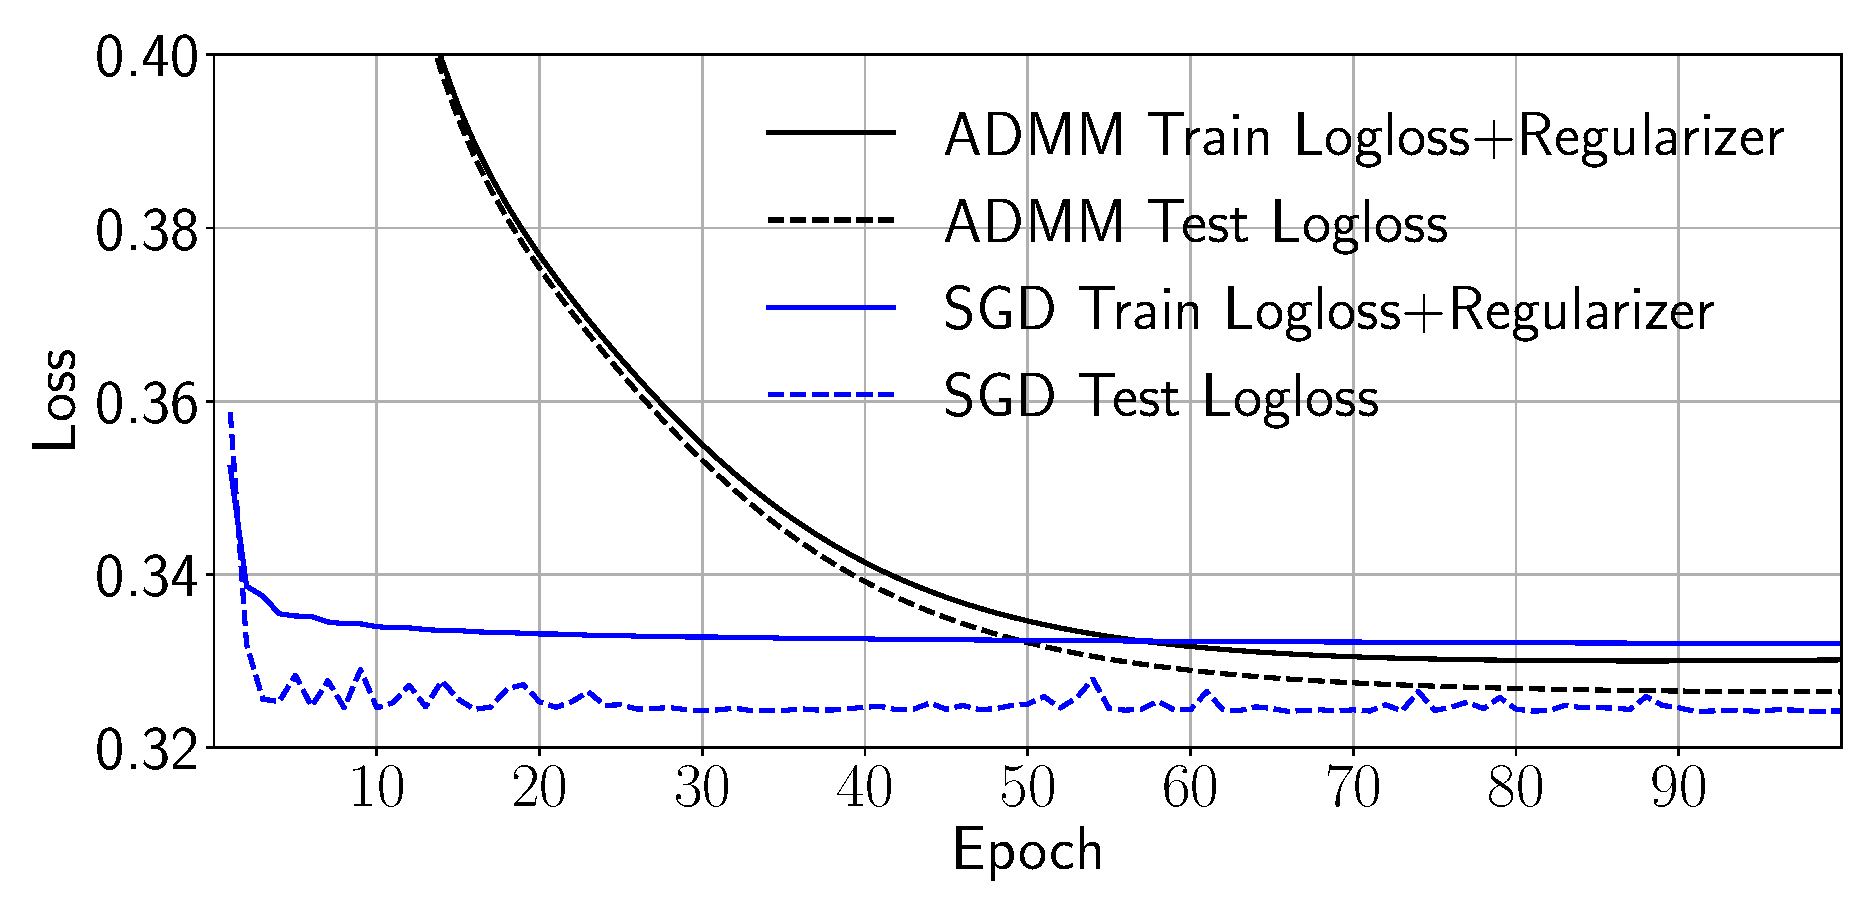
\includegraphics[width=3.4in]{figures/a9a_loss_vs_epoch}
    \label{fig:a9a_loss_vs_epoch}
    }
    % \hspace{-3.5mm}
    \subfigure[Test log loss under different noise levels]{
    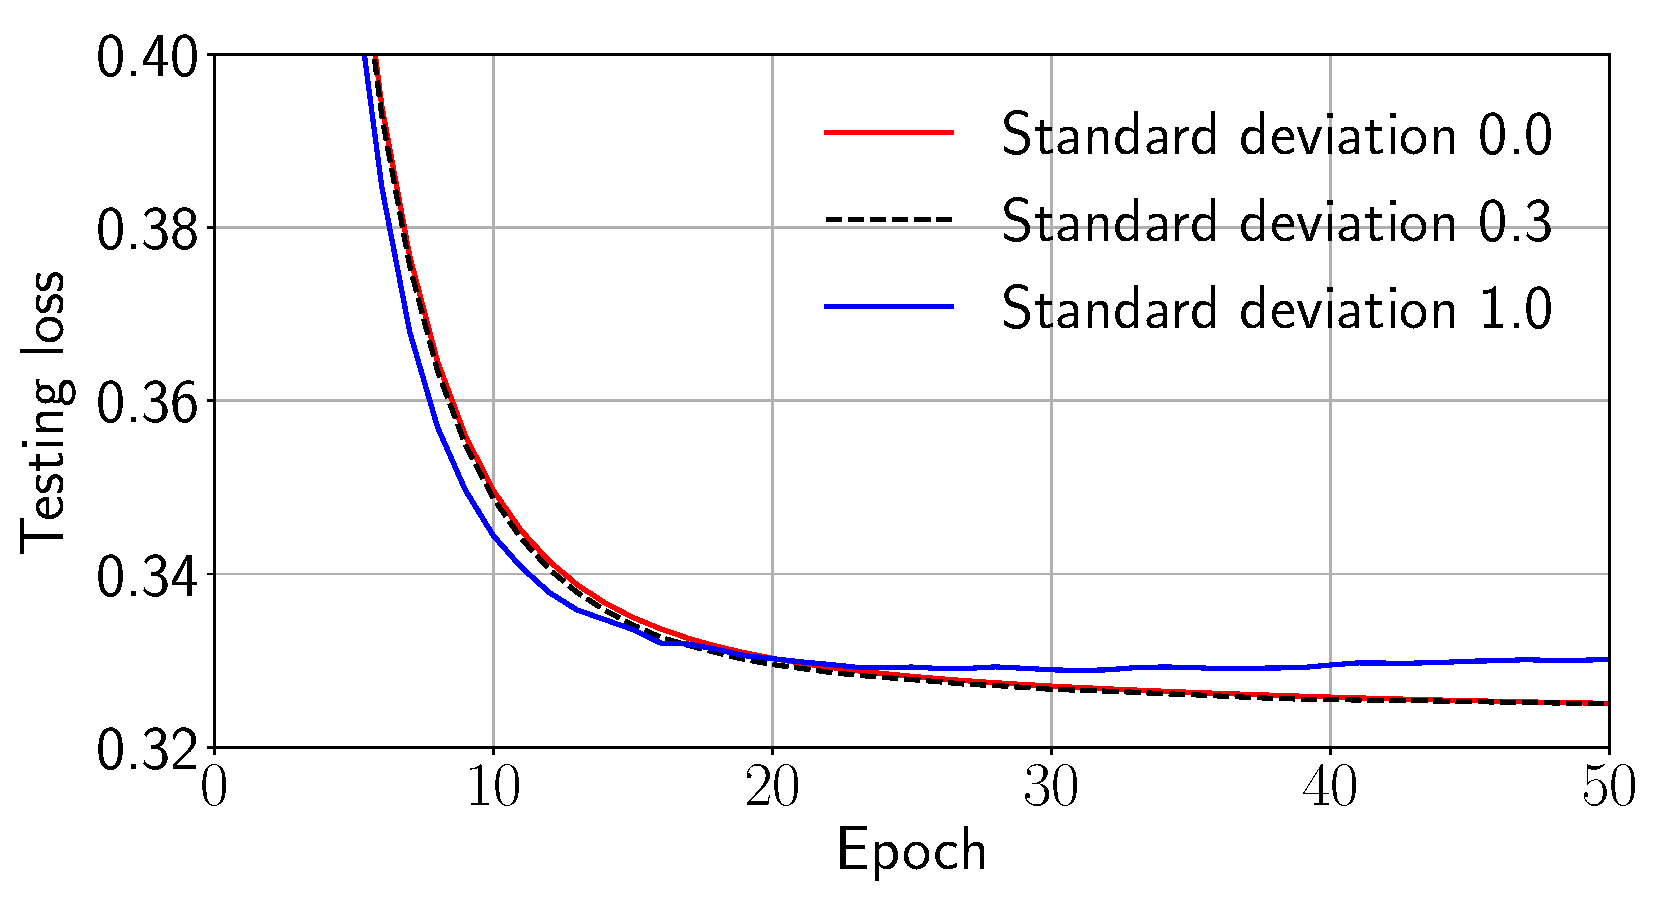
\includegraphics[width=3.4in]{figures/a9a_test_loss_vs_epoch_vary_noise}
    \label{fig:a9a_loss_vs_time}
    }
    % \vspace{-3.5mm}
    \caption{Performance over the \emph{a9a} data set with 32561 training samples, 16281 testing samples and 123 features.}
    \label{fig:a9a_train}
    \vspace{-4mm}
\end{figure*}

\begin{figure*}[t]
    \centering
    % \vspace{-5mm}
    \subfigure[Loss vs. epoch]{
    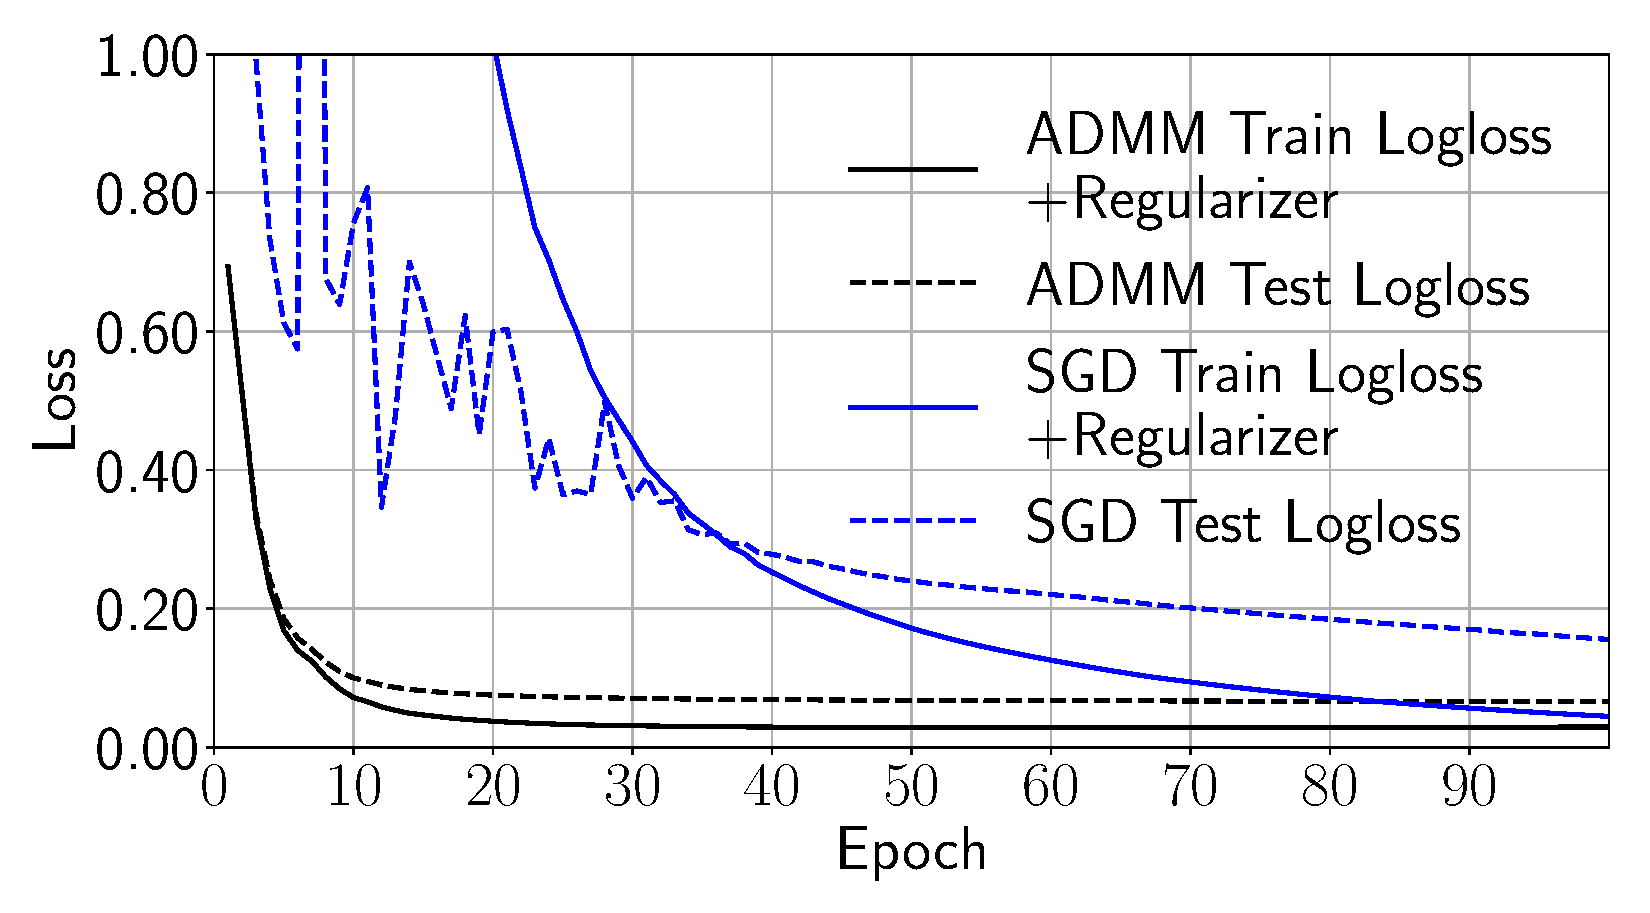
\includegraphics[width=3.4in]{figures/gisette_loss_vs_epoch}
    \label{fig:gisette_loss_vs_epoch}
    }
    % \hspace{-3.5mm}
    \subfigure[Test log loss under different noise levels]{
    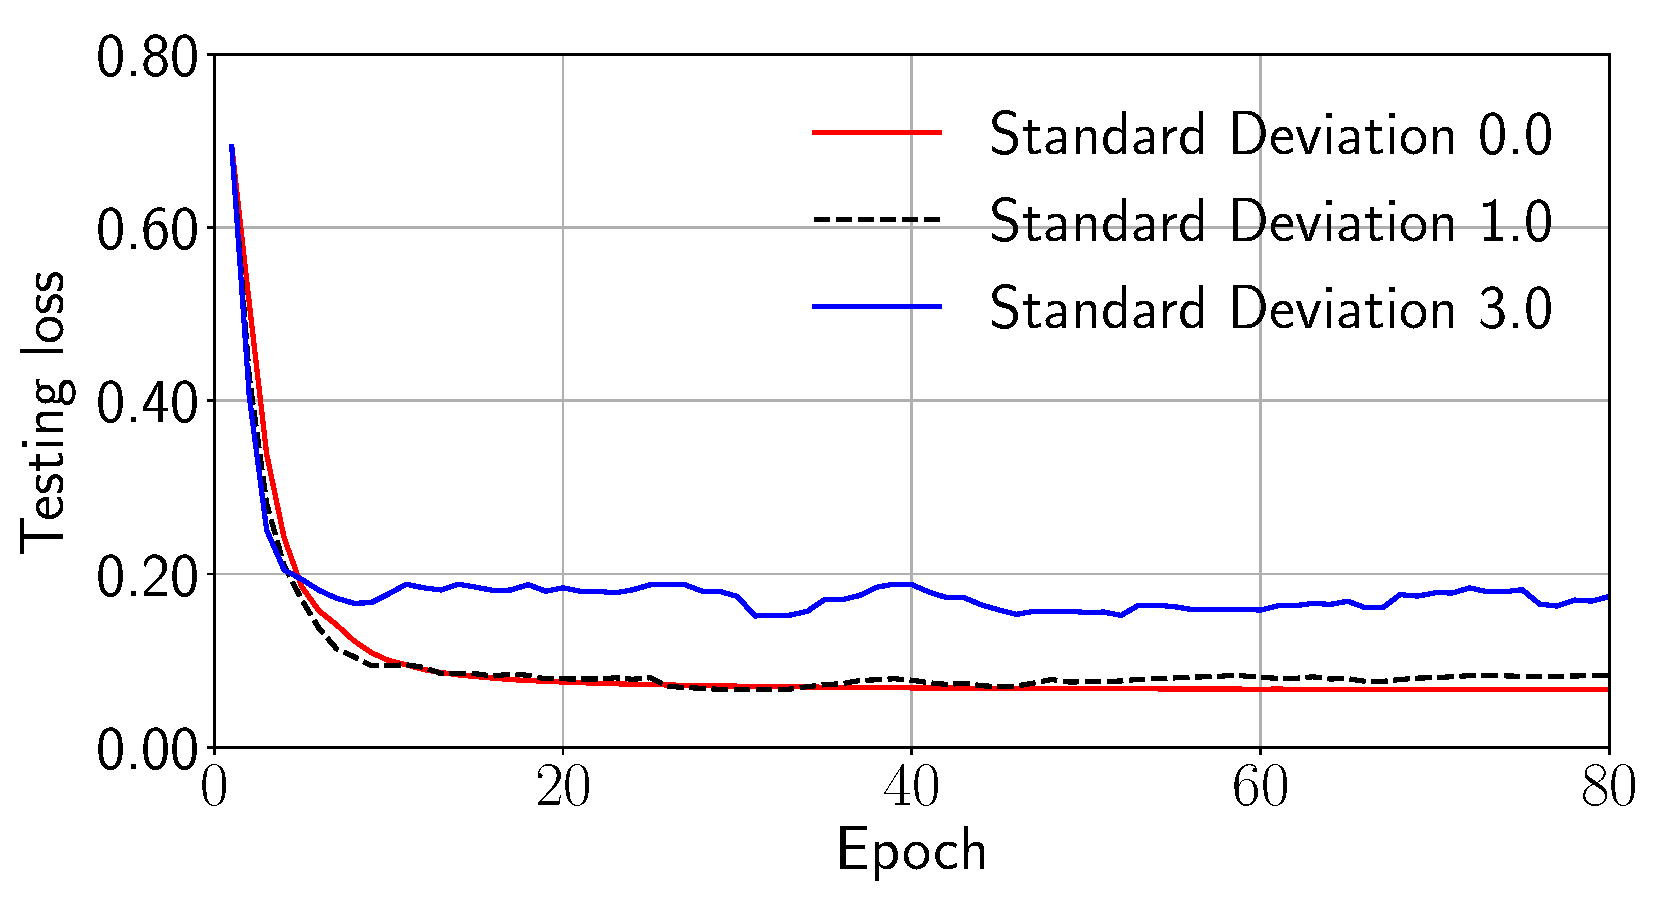
\includegraphics[width=3.4in]{figures/gisette_test_loss_vs_epoch_vary_noise}
    \label{fig:gisette_loss_vs_time}
    }
    % \vspace{-3.5mm}
    \caption{Performance over the \emph{gisette} data set with 6000 training samples, 1000 testing samples and 5000 features.}
    \label{fig:gisette_train}
    \vspace{-4mm}
\end{figure*}

\begin{figure*}[t]
    \centering
    % \vspace{-5mm}
    \subfigure[\emph{a9a} data set]{
    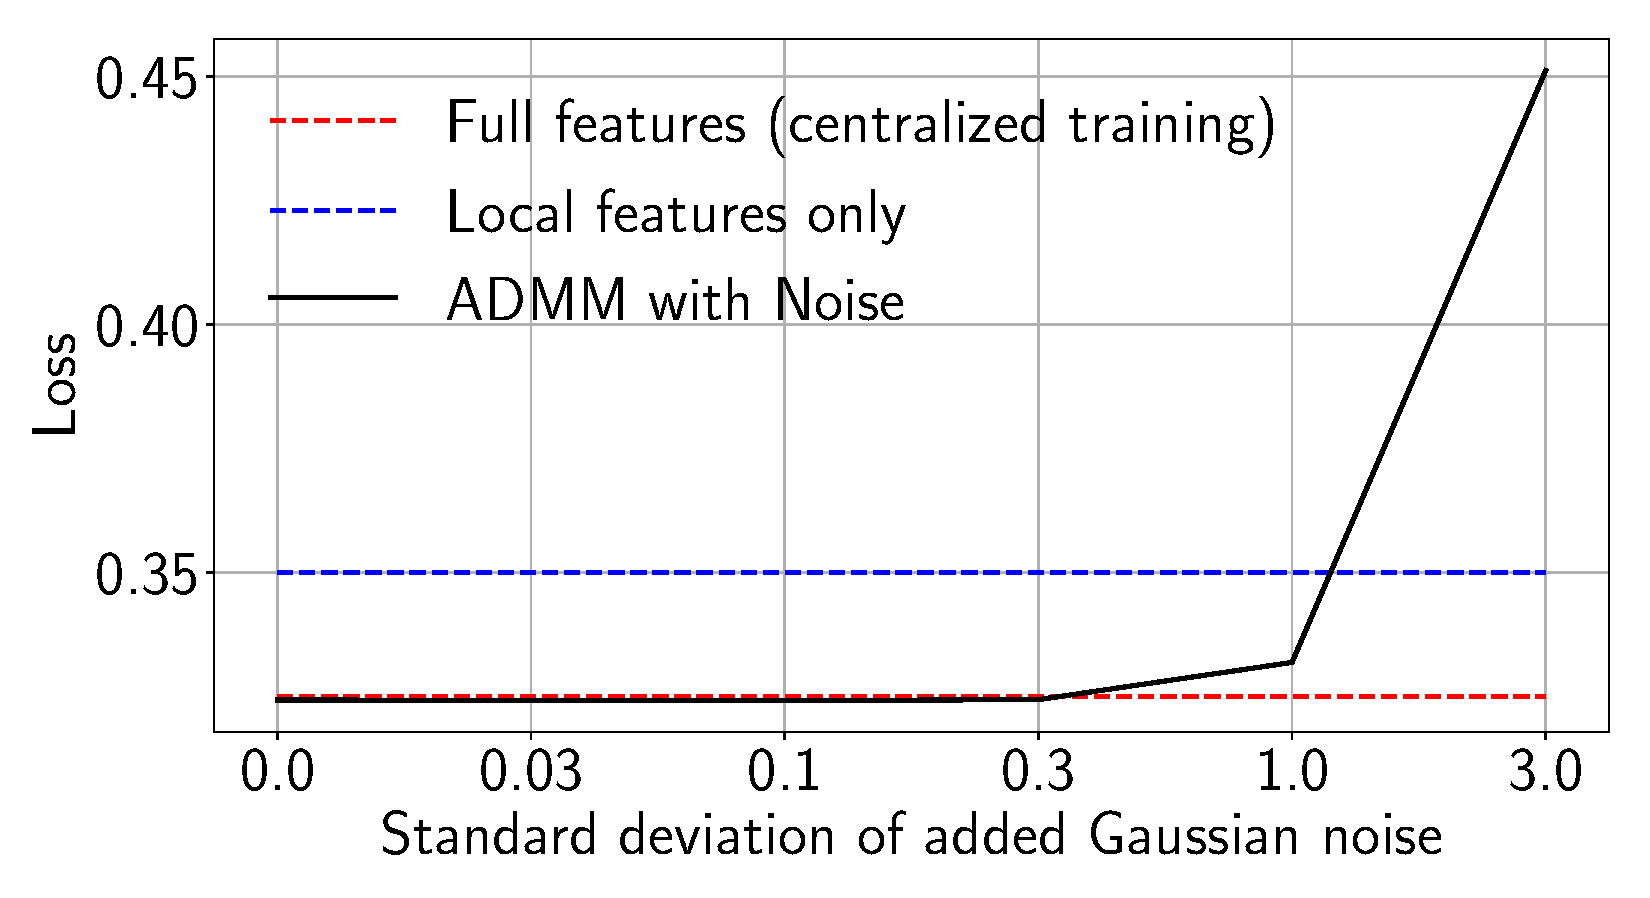
\includegraphics[width=3.4in]{figures/a9a_test_loss_vs_noise}
    \label{fig:a9a_test_loss_vs_noise}
    }
    % \hspace{-3.5mm}
    \subfigure[\emph{gisette} data set]{
    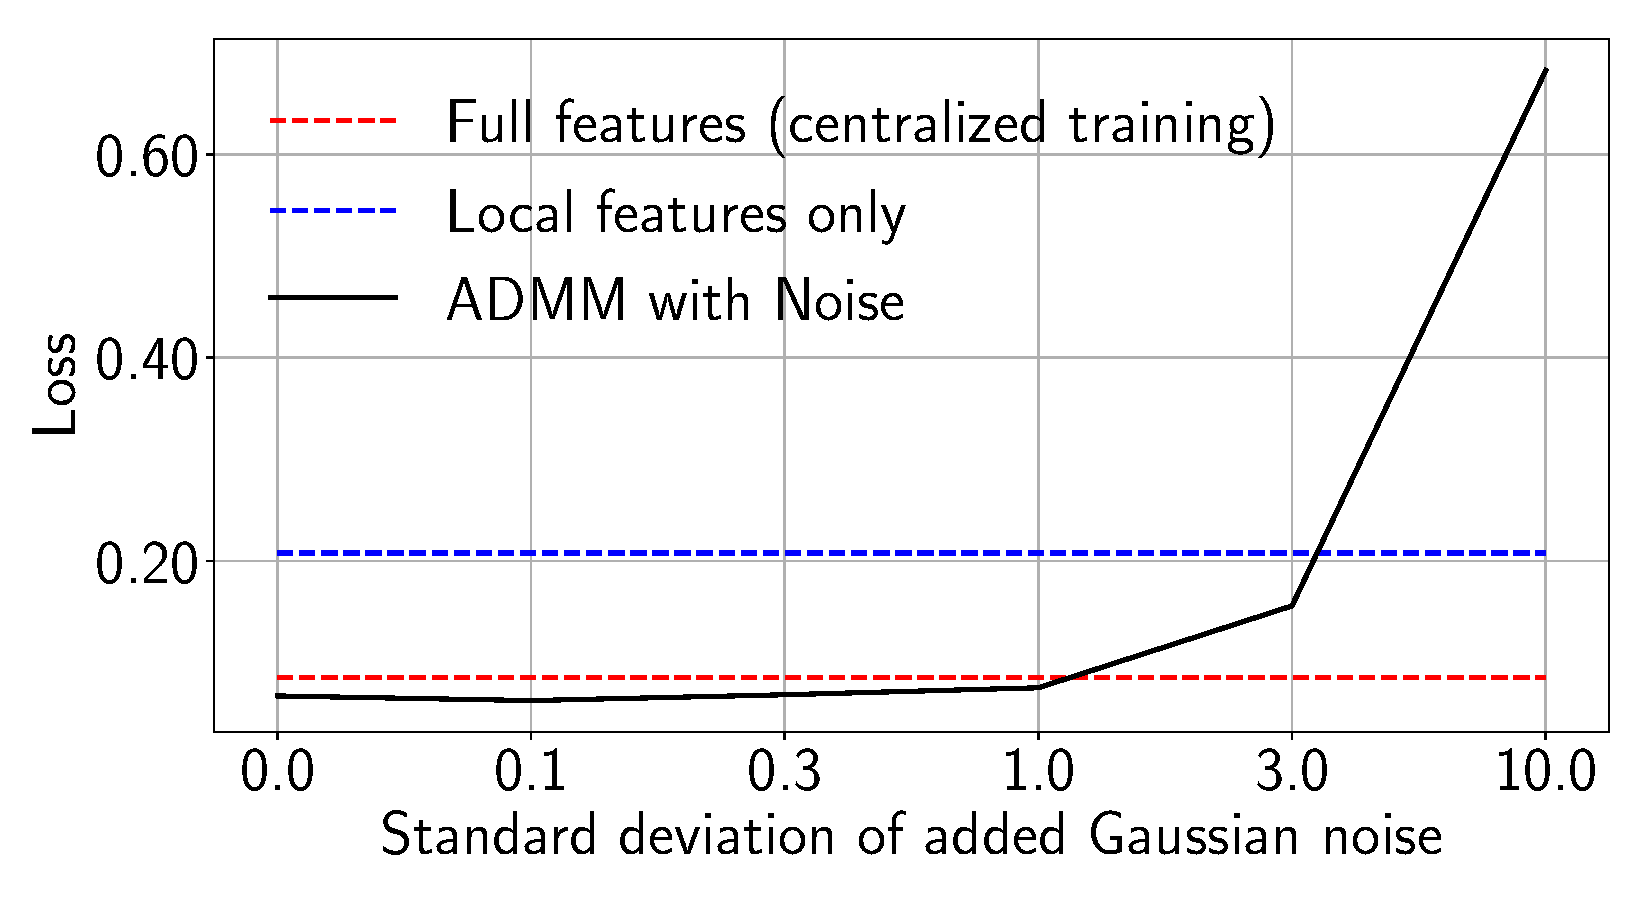
\includegraphics[width=3.4in]{figures/gisette_test_loss_vs_noise}
    \label{fig:gisette_test_loss_vs_noise}
    }
    % \vspace{-3.5mm}
    \caption{Test performance for ADMM under different levels of added noise.}
    \label{fig:loss_vs_noise}
     \vspace{-4mm}
\end{figure*}

We test our algorithm by training $l_2$-norm regularized logistic regression on two popular public datasets, namely, \emph{a9a} from UCI \cite{Dua:2019} and \emph{giette} \cite{guyon2005result}. We get the datasets from \cite{Liblinear:2019} so that we follow the same preprocessing procedure listed there. \emph{a9a} dataset is $4$ MB and contains 32561 training samples, 16281 testing samples and 123 features. We divide the dataset into two parts, with the first part containing the first 66 features and the second part remaining 57 features. The first part is regarded as the local party who wishes to improve its prediction model with the help of data from the other party. On the other hand, \emph{gisette} dataset is $297$ MB and contains 6000 training samples, 1000 testing samples and 5000 features. Similarly, we divide the features into 3 parts, the first 2000 features being the first part regarded as the local data, the next 2000 features being the second part, and the remaining 1000 as the third part. Note that \emph{a9a} is small in terms of the number of features and \emph{gisette} has a relatively higher dimensional feature space.

A prototype system is implemented in \emph{Python} to verify our proposed algorithm. Specifically, we use optimization library from \emph{scipy} to handle the optimization subproblems. We apply L-BFGS-B algorithm to do the $x$ update in \eqref{eq:pal_algo_x} and entry-wise optimization for $z$ in \eqref{eq:pal_algo_z}. We run the experiment on a machine equipped with Intel(R) Core(TM) i9-9900X CPU @ 3.50GHz and 128 GB of memory. 

We compare our algorithm against an SGD based algorithm proposed in \cite{hu2019fdml}.
We keep track of the training objective value (log loss plus the $l_2$ regularizer), the testing log loss for each epoch for different datasets and parameter settings. We also test our algorithm with different levels of Gaussian noise added. In the training procedure, we initialize the elements in $x$, $y$ and $z$ with $0$ while we initialize the parameter for the SGD-based algorithm with random numbers.

Fig.~\ref{fig:a9a_train} and Fig.~\ref{fig:gisette_train} show a typical trace of the training objective and testing log loss against epochs for \emph{a9a} and \emph{gisette}, respectively. On \emph{a9a}, the ADMM algorithm is slightly slower than the SGD based algorithm, while they reach the same testing log loss in the end. On \emph{gisette}, the SGD based algorithm converges slowly while the ADMM algorithm is efficient and robust. The testing log loss from the ADMM algorithm quickly converges to 0.08 after a few epochs, but the SGD based algorithm converges to only 0.1 with much more epochs. This shows that the ADMM algorithm is superior when the number of features is large.
In fact, for each epoch, the $x$ update is a trivial quadratic program and can be efficiently solved numerically. The $z$ update contains optimization over computationally expensive functions, but for each sample, it is always an optimization over a single scalar so that it can be solved efficiently via scalar optimization and scales with the number of features. 

Moreover, Corollary~\ref{theorem:overall_privacy} implies that the total differential privacy guarantee will be stronger if the number of epochs required for convergence is less. The fast convergence rate of the ADMM sharing algorithm also makes it more appealing to achieve differential privacy guarantees than SGD, especially in the case of wide features (\emph{gisette}).

Fig.~\ref{fig:loss_vs_noise} shows the testing loss for ADMM with different levels of Gaussian noise added. The other two baselines are the logistic regression model trained over all the features (in a centralized way) and that trained over only the local features in the first party. The baselines are trained with the built-in logistic regression function from \emph{sklearn} library. We can see that there is a significant performance boost if we employ more features to help training the model on Party 1. Interestingly, in Fig.~\ref{fig:gisette_test_loss_vs_noise}, the ADMM sharing has even better performance than the baseline trained with all features with \emph{sklearn}. It further shows that the ADMM sharing is better at datasets with a large number of features. 

Moreover, after applying moderate random perturbations, the proposed algorithm can still converge in a relatively small number of epochs, as Fig.~\ref{fig:a9a_loss_vs_time} and Fig.~\ref{fig:gisette_loss_vs_time} suggest, although too much noise may ruin the model.
%Thus, we can still achieve better performance than using local features only, although too much noise will ruin the model. 
Therefore, ADMM sharing algorithm under moderate perturbation can improve the local model and the privacy cost is well contained as the algorithm converges in a few epochs.



\section{Conclusion}

We study learning over distributed features (vertically partitioned data) where none of the parties shall share the local data. %The motivation is in contrast to the most existing literature on collaborative and distributed machine learning where the data samples (but not the features) are assumed to distribute and work in a data-parallel fashion. 
We propose the parallel ADMM sharing algorithm to solve this challenging problem where only intermediate values are shared, without even sharing model parameters. To further protect the data privacy, we apply the differential privacy technique in the training procedure to derive a privacy guarantee within $T$ epochs. 
We implement a prototype system and evaluate the proposed algorithm on two representative datasets in risk minimization. The result shows that the ADMM sharing algorithm converges efficiently, especially on dataset with large number of features. Furthermore, the differentially private ADMM algorithm yields better prediction accuracy than model trained from only local features while ensuring a certain level of differential privacy guarantee. 

\bibliographystyle{aaai}
\bibliography{main}

\newpage
\clearpage
\onecolumn
\newpage
\section{Supplementary Materials}
\subsection{Proof of Theorem~\ref{theo:convergence}}
To help theoretical analysis, we denote the objective functions in \eqref{eq:pal_algo_x} and \eqref{eq:pal_algo_z} as
\begin{align}
    & g_m(x_m) = \lambda R_m(x_m) + \langle y^t, \mathcal{D}_mx_m\rangle + \frac{\rho}{2}\big\|\sum_{\substack{k=1\\k\neq m}}^{M} \mathcal{D}_kx_k^t+ \mathcal{D}_mx_m - z^t\big\|^2,\nonumber\\
    & h(z) = l(z)  - \langle y^t, z \rangle + \frac{\rho}{2} \big\|\sum_{m=1}^{M}\mathcal{D}_mx_m^{t+1} - z\big\|^2,
\end{align}
correspondingly. We prove the following four lemmas to help prove the theorem. 
\begin{lemma}\label{lemma:y_diff_bound}
Under Assumption~\ref{theo:assumptions_pri}, we have
\[
    \nabla l(z^{t+1}) = y^{t+1},
\]
and
\[
    \|y^{t+1} - y^t\|^2 \le L^2\|z^{t+1} - z^{t}\|^2.
\]
\end{lemma}
{\bf Proof.} By the optimality in \eqref{eq:pal_algo_z}, we have
\begin{align}
    \nabla l(z^{t+1}) - y^t + \rho\big(z^{t+1} - \sum_{m=1}^{M} \mathcal{D}_mx_m^{t+1}\big) = 0.\nonumber
\end{align}
Combined with \eqref{eq:pal_algo_y}, we can get
\begin{align}
    \nabla l(z^{t+1}) = y^{t+1}.
\end{align}
Combined with Assumption~\ref{theo:assumptions_pri}.\ref{item:assum_1_pri}, we have
\begin{align}
\|y^{t+1} - y^{t}\|^2 = \|\nabla l(z^{t+1}) - \nabla l(z^{t})\|^2 \le L^2\|z^{t+1} - z^t\|^2.
\end{align}
\hfill$\square$

\begin{lemma}\label{lemma:algebra_1}
    We have 
    \begin{align}
        & \big(\|\sum_{m=1}^{M} x_m^{t+1} - z\|^2 - \|\sum_{m=1}^{M} x_m^{t} - z\|^2\big) - \sum_{m=1}^{M}\big(\|\sum_{\substack{k=1\\k\neq m}}^M x_k^{t} + x_m^{t+1} - z\|^2 - \|\sum_{m=1}^{M} x_m^{t} - z\|^2\big)\nonumber\\
        \le & \sum_{m=1}^{M} \|x_m^{t+1} - x_m^{t}\|^2.
    \end{align}
\end{lemma}
{\bf Proof.}
\begin{align}
    \text{LHS} = & \big(\sum_{m=1}^{M}(x_m^{t+1} + x_m^{t}) - 2z\big)\top(\sum_{m=1}^{M} x_m^{t+1} - \sum_{m=1}^{M} x_m^t) - \sum_{m=1}^{M} \big(\sum_{\substack{k=1\\k\neq m}}^M2x_k^t + x_m^t + x_m^{t+1} -2z\big)\top(x_m^{t+1} - x_m^t)\nonumber\\
    = & - \sum_{m=1}^{M} \sum_{\substack{k=1\\k\neq m}}^M(x_k^{t+1} - x_k^{t})\top(x_m^{t+1} - x_m^t)\nonumber\\
    = & - \|\sum_{m=1}^{M} (x_m^{t+1} - x_m^{t})\|^2 + \sum_{m=1}^{M} \|x_m^{t+1} - x_m^{t}\|^2\nonumber\\
    \le & \sum_{m=1}^{M} \|x_m^{t+1} - x_m^{t}\|^2.\nonumber
\end{align}
\hfill$\square$

\begin{lemma}\label{lemma:L_iter_diff}
Suppose Assumption~\ref{theo:assumptions_pri} holds. We have
\begin{align}
    & \mathcal{L}(\{x_m^{t+1}\},z^{t+1};y^{t+1}) - \mathcal{L}(\{x_m^{t}\},z^{t};y^{t})\nonumber\\
    & \le \sum_{m=1}^{M} -\left(\frac{\gamma_m(\rho)}{2}-\sigma_{\text{max}}(\mathcal{D}_m^\top \mathcal{D}_m)\right)\|x_m^{t+1} - x_m^t\|^2 - \left(\frac{\gamma(\rho)}{2} - \frac{L^2}{\rho}\right)\|z^{t+1} - z^t\|^2. \nonumber
\end{align}
\end{lemma}
{\bf Proof.} The LFH can be decomposed into two parts as
\begin{align}
    & \mathcal{L}(\{x_m^{t+1}\},z^{t+1};y^{t+1}) - \mathcal{L}(\{x_m^{t}\},z^{t};y^{t})\nonumber\\
    = & \big(\mathcal{L}(\{x_m^{t+1}\},z^{t+1};y^{t+1}) - \mathcal{L}(\{x_m^{t+1}\},z^{t+1};y^{t})\big)\nonumber\\
    & + \big(\mathcal{L}(\{x_m^{t+1}\},z^{t+1};y^{t}) - \mathcal{L}(\{x_m^{t}\},z^{t};y^{t})\big). \label{eq:proof_diff_L_0_pal}
\end{align}
For the first term, we have
\begin{align}
    & \mathcal{L}(\{x_j^{t+1}\},z^{t+1};y^{t+1}) - \mathcal{L}(\{x_j^{t+1}\},z^{t+1};y^{t})\nonumber\\
    = & \langle y^{t+1} - y^t , \sum_jD_jx_j^{t+1} - z^{t+1}\rangle\nonumber\\
    = & \frac{1}{\rho}\|y^{t+1} - y^t\|^2\quad\text{(by \eqref{eq:pal_algo_y})}\nonumber\\
    = & \frac{L^2}{\rho}\|z^{t+1} - z^t\|^2\quad\text{(by Lemma~\ref{lemma:y_diff_bound})}\label{eq:proof_diff_L_1_pal}.
\end{align}
For the second term, we have
\begin{align}
    & \mathcal{L}(\{x_m^{t+1}\},z^{t+1};y^{t}) - \mathcal{L}(\{x_m^{t}\},z^{t};y^{t})\nonumber\\
    = & \mathcal{L}(\{x_m^{t+1}\},z^{t+1};y^{t}) - \mathcal{L}(\{x_m^{t}\},z^{t+1};y^{t}) + \mathcal{L}(\{x_m^{t}\},z^{t+1};y^{t}) - \mathcal{L}(\{x_m^{t}\},z^{t};y^{t})\nonumber\\
    \le & \bigg(\big(\lambda \sum_{m=1}^{M}R_m(x_m^{t+1}) + \langle y^t, \sum_{m=1}^{M}\mathcal{D}_mx_m^{t+1}\rangle + \frac{\rho}{2}\big\|\sum_{k=1}^M \mathcal{D}_kx_k^{t+1} - z^{t+1}\big\|^2\big)\nonumber\\
    & - \big(\lambda \sum_{m=1}^{M}R_m(x_m^{t}) + \langle y^t, \sum_{m=1}^{M}\mathcal{D}_mx_m^{t}\rangle + \frac{\rho}{2}\big\|\sum_{k=1}^M \mathcal{D}_kx_k^{t} - z^{t+1}\big\|^2\big)\bigg)\nonumber\\
    & + \bigg(\big(l(z^{t+1}) -\langle y^t, z^{t+1}\rangle + \frac{\rho}{2} \big\|\sum_{m=1}^{M} \mathcal{D}_mx_m^{t+1} - z^{t+1}\big\|^2\big)-\big(l(z^{t}) -\langle y^t, z^{t}\rangle+ \frac{\rho}{2} \big\|\sum_{m=1}^{M} \mathcal{D}_mx_m^{t+1} - z^{t}\big\|^2\big)\bigg)\nonumber\\
    \le & \sum_{m=1}^{M} \bigg(\big(\lambda R_m(x_m^{t+1}) + \langle y^t, \mathcal{D}_mx_m^{t+1}\rangle + \frac{\rho}{2}\big\|\sum_{\substack{k=1\\k\neq m}}^M\mathcal{D}_kx_k^{t} + \mathcal{D}_mx_m^{t+1} - z^{t+1}\big\|^2\big)\nonumber\\
    & - \big(\lambda R_m(x_m^{t}) + \langle y^t, \mathcal{D}_mx_m^{t}\rangle + \frac{\rho}{2}\big\|\sum_{k=1}^{M}\mathcal{D}_kx_k^{t} - z^{t+1}\big\|^2\big)\bigg)+\sum_{m=1}^{M} \|\mathcal{D}_m(x_m^{t+1} - x_m^t)\|^2\nonumber\\
    & + \bigg(\big(l(z^{t+1}) -\langle y^t, z^{t+1}\rangle + \frac{\rho}{2} \big\|\sum_{m=1}^{M} \mathcal{D}_mx_m^{t+1} - z^{t+1}\big\|^2\big)\nonumber\\
    & -\big(l(z^{t}) -\langle y^t, z^{t}\rangle+ \frac{\rho}{2} \big\|\sum_{m=1}^{M} \mathcal{D}_mx_m^{t+1} - z^{t}\big\|^2\big)\bigg)\quad\text{(by Lemma~\ref{lemma:algebra_1})}\nonumber\\
    = & \sum_{m=1}^{M} \big(g_m(x_m^{t+1}) - g_m(x_m^t)\big) + (h(z^{t+1}) - h(z^T)))+\sum_{m=1}^{M} \|\mathcal{D}_m(x_m^{t+1} - x_m^t)\|^2\nonumber\\
    \le & \sum_{m=1}^{M} \big(\langle \nabla g_m(x_m^{t+1}), x_m^{t+1}-x_m^t\rangle - \frac{\gamma_m(\rho)}{2}\|x_m^{t+1}-x_m^t\|^2\big) + \langle\nabla h(z^{t+1}), z^{t+1} - z^t\rangle - \frac{\gamma(\rho)}{2}\|z^{t+1} - z^t\|^2\nonumber\\
    & +\sum_{m=1}^{M} \|\mathcal{D}_m(x_m^{t+1} - x_m^t)\|^2\quad\text{(by strongly convexity from Assumption~\ref{theo:assumptions_pri}.\ref{item:assum_2_pri})}\nonumber
\end{align}
\begin{align}
    \le & -\sum_{m=1}^{M}\frac{\gamma_m(\rho)}{2}\|x_m^{t+1}-x_m^t\|^2 - \frac{\gamma(\rho)}{2}\|z^{t+1} - z^t\|^2+\sum_{m=1}^{M}\|\mathcal{D}_m(x_m^{t+1} - x_m^t)\|^2\nonumber\\
    & \text{(by optimality condition for subproblem in \eqref{eq:pal_algo_x} and \eqref{eq:pal_algo_z})}\nonumber\\
    \le & \sum_{m=1}^{M} -\left(\frac{\gamma_m(\rho)}{2}-\sigma_{\text{max}}(\mathcal{D}_m^\top \mathcal{D}_m)\right)\|x_m^{t+1} - x_m^t\|^2 - \frac{\gamma(\rho)}{2}\|z^{t+1} - z^t\|^2.\label{eq:proof_diff_L_2_pal}
\end{align}
Note that we have abused the notation $\nabla g_m(x_m)$ and denote it as the subgradient when $g$ is non-smooth but convex.
Combining \eqref{eq:proof_diff_L_0_pal}, \eqref{eq:proof_diff_L_1_pal} and \eqref{eq:proof_diff_L_2_pal}, the lemma is proved.\hfill$\square$

\begin{lemma}\label{lemma:L_lower_bound}
    Suppose Assumption~\ref{theo:assumptions_pri} holds. Then the following limit exists and is bounded from below:
    \begin{align}
        \underset{t\rightarrow\infty}{\text{lim}} \mathcal{L}(\{x^{t+1}\}, z^{t+1}; y^{t+1}).
    \end{align}
\end{lemma}
{\bf Proof.}
\begin{align}
    & \mathcal{L}(\{x^{t+1}\}, z^{t+1}; y^{t+1} )\nonumber\\
    = & l(z^{t+1}) + \lambda\sum_{m=1}^{M} R_m(x_m^{t+1}) + \langle y^{t+1}, \sum_{m=1}^{M}\mathcal{D}_m x_m^{t+1} - z^{t+1}\rangle + \frac{\rho}{2}\|\mathcal{D}_m x_m^{t+1} - z^{t+1}\|^2\nonumber\\
    = &\lambda\sum_{m=1}^{M} R_m(x_m^{t+1}) + l(z^{t+1}) + \langle \nabla l(z^{t+1}), \sum_{m=1}^{M}\mathcal{D}_m x_m^{t+1} - z^{t+1}\rangle + \frac{\rho}{2}\|\mathcal{D}_m x_m^{t+1} - z^{t+1}\|^2\quad\text{(by Lemma~\ref{lemma:y_diff_bound})}\nonumber\\
    \ge & \lambda\sum_{m=1}^{M} R_m(x_m^{t+1}) + l(\sum_{m=1}^{M}\mathcal{D}_m x_m^{t+1}) + \frac{\rho-L}{2}\|\mathcal{D}_m x_m^{t+1} - z^{t+1}\|^2.\quad%\text{(from Assumption~\ref{theo:assumptions_pal}.\ref{item:assum_1_pal})}
\end{align}
Combined with Assumption~\ref{theo:assumptions_pri}.\ref{item:assum_3_pri}, $\mathcal{L}(\{x^{t+1}\}, z^{t+1}; y^{t+1})$ is lower bounded. Furthermore, by Assumption~\ref{theo:assumptions_pri}.\ref{item:assum_2_pri} and Lemma~\ref{lemma:L_iter_diff}, $\mathcal{L}(\{x^{t+1}\}, z^{t+1}; y^{t+1})$ is decreasing. These complete the proof. \hfill$\square$

Now we are ready for the proof.

{\bf Part 1. } By Assumption~\ref{theo:assumptions_pri}.\ref{item:assum_2_pri}, Lemma~\ref{lemma:L_iter_diff} and Lemma~\ref{lemma:L_lower_bound}, we have
\begin{align}
    & \|x_m^{t+1} - x_m^t\|\rightarrow 0\quad\forall m=1,2,\ldots, M,\nonumber\\
    & \|z^{t+1} - z^t\|\rightarrow 0.\nonumber
\end{align}
Combined with Lemma~\ref{lemma:y_diff_bound}, we have
\begin{align}
    \|y^{t+1}-y^t\|^2\rightarrow 0.\nonumber
\end{align}
Combined with~\eqref{eq:pal_algo_y}, we complete the proof for Part 1.

{\bf Part 2.} Due to the fact that $\|y^{t+1}-y^t\|^2\rightarrow 0$, by taking limit in \eqref{eq:pal_algo_y}, we can get \eqref{eq:cond_primal}.

At each iteration $t+1$, by the optimality of the subproblem in \eqref{eq:pal_algo_z}, we have
\begin{align}
    \nabla l(z^{t+1}) - y^t + \rho (z^{t+1} - \sum_{m=1}^{M}\mathcal{D}_mx_m^{t+1}) = 0.
\end{align}
Combined with \eqref{eq:cond_primal} and taking the limit, we get \eqref{eq:cond_dual}.

Similarly, by the optimality of the subproblem in \eqref{eq:pal_algo_x}, for $\forall m\in\mathcal{M}$ there exists $\eta_m^{t+1}\in\partial R_m(x_m^{t+1})$, such that
\begin{align}
    \big\langle x_m-x_m^{t+1}, \lambda \eta_m^{t+1} + \mathcal{D}_m^Ty^t + \rho \mathcal{D}_m^T\big(\sum_{\substack{k=1\\k\le m}}^M \mathcal{D}_kx_k^{t+1} + \sum_{\substack{k=1\\k>j}}^M \mathcal{D}_kx_k^{t} - z^{t}\big)\big\rangle \ge 0\quad \forall x_m\in X_m.
\end{align}
Since $R_m$ is convex, we have
\begin{align}
    \lambda R_m(x_m) - \lambda R_m(x_m^{t+1}) + \big\langle x-x_m^{t+1}, \mathcal{D}_m^\top y^t + \rho\big(\sum_{\substack{k=1\\k\le m}}^M \mathcal{D}_kx_k^{t+1} + \sum_{\substack{k=1\\k>j}}^M \mathcal{D}_kx_k^{t} - z^{t}\big)^T \mathcal{D}_j\big\rangle \ge 0\quad \forall x_m\in X_m.
\end{align}
Combined with \eqref{eq:cond_primal} and the fact $\|x_m^{t+1} - x_m^{t}\|\rightarrow 0$, by taking the limit, we get
\begin{align}
    \lambda R_m(x_m) - \lambda R_m(x_m^*) + \big\langle x-x_m^{*}, \mathcal{D}_m^\top y^* \big\rangle \ge 0\quad \forall x_m\in X_m, \forall m,
\end{align}
which is equivalent to
\begin{align}
    \lambda R_m(x) + \big\langle y^*, \mathcal{D}_mx \big\rangle- \lambda R_m(x_m^*) - \big\langle y^*, \mathcal{D}_mx_m^{*} \big\rangle \ge 0\quad \forall x\in X_m, \forall m.
\end{align}
And we can get the result in \eqref{eq:cond_x_opt_conv}. \\
When $m\not\in\mathcal{M}$, we have
\begin{align}
    \big\langle x_m-x_m^{t+1}, \lambda \nabla R_m(x_m^{t+1}) + \mathcal{D}_m^\top y^t + \rho\big(\sum_{\substack{k=1\\k\le m}}^M \mathcal{D}_kx_k^{t+1} + \sum_{\substack{k=1\\k>j}}^M \mathcal{D}_kx_k^{t} - z^{t}\big)^T \mathcal{D}_m\big\rangle \ge 0\quad \forall x_m\in X_m.
\end{align}
Taking the limit and we can get \eqref{eq:cond_x_opt_nonconv}.

{\bf Part 3.} We first show that there exists a limit point for each of the sequences $\{x_m^t\}$, $\{z^t\}$ and $\{y^t\}$. Since $X_m, \forall m$ is compact, $\{x_m^t\}$ must have a limit point. With Theorem~\ref{theo:convergence}.\ref{item:primal_cond_limit}, we can get that $\{z^t\}$ is also compact and has a limit point. Furthermore, with Lemma~\ref{lemma:y_diff_bound}, we can get $\{y^t\}$ is also compact and has a limit point.

We prove Part 3 by contradiction. Since $\{x_m^t\}$, $\{z^t\}$ and $\{y^t\}$ lie in some compact set, there exists a subsequence $\{x_m^{t_k}\}$, $\{z^{t_k}\}$ and $\{y^{t_k}\}$, such that
\begin{align}
    (\{x_m^{t_k}\}, z^{t_k}; y^{t_k})\rightarrow (\{\hat{x}_m\}, \hat{z}; \hat{y}), \label{eq:subseq_limit}
\end{align}
where $(\{\hat{x}_m\}, \hat{z}; \hat{y})$ is some limit point and by part 2, we have $(\{\hat{x}_m\}, \hat{z}; \hat{y})\in Z^*$. Suppose that $\{\{x_m^t\}, z^t; y^t\}$ does not converge to $Z^*$, since $(\{x_m^{t_k}\}, z^{t_k}; y^{t_k})$ is a subsequence of it, there exists some $\gamma>0$, such that
\begin{align}
    \underset{k\rightarrow\infty}{\lim}\quad\text{dist}\big((\{x_m^{t_k}\}, z^{t_k}; y^{t_k});Z^*\big)=\gamma>0.\label{eq:suppose}
\end{align}
From \eqref{eq:subseq_limit}, there exists some $J(\gamma)>0$, such that
\begin{align}
        \|(\{x_m^{t_k}\}, z^{t_k}; y^{t_k})- (\{\hat{x}_m\}, \hat{z}; \hat{y})\|\le\frac{\gamma}{2}, \quad\forall k\ge J(\gamma).
\end{align}
Since $(\{\hat{x}_m\}, \hat{z}; \hat{y})\in Z^*$, we have
\begin{align}
    \text{dist}\big((\{x_m^{t_k}\}, z^{t_k}; y^{t_k});Z^*\big) \le \text{dist}\big((\{x_m^{t_k}\}, z^{t_k}; y^{t_k});  (\{\hat{x}_m\}, \hat{z}; \hat{y})\big).
\end{align}
From the above two inequalities, we must have
\begin{align}
    \text{dist}\big((\{x_m^{t_k}\}, z^{t_k}; y^{t_k});Z^*\big)\le\frac{\gamma}{2},\quad\forall k\ge J(\gamma),
\end{align}
which contradicts to \eqref{eq:suppose}, completing the proof.
\hfill$\square$

\subsection{Proof of Theorem~\ref{theo:iter_complexity}}
We first show an upper bound for $V^t$.

1. Bound for $\tilde{\nabla}_{x_m} \mathcal{L}(\{x_m^t\}, z^t; y^t)$. When $m\in\mathcal{M}$, from the optimality condition in \eqref{eq:pal_algo_x}, we have
\begin{align}
    0 \in \lambda\partial_{x_m}R_j(x_m^{t+1}) + \mathcal{D}^\top y^t + \rho \mathcal{D}_j^\top \big(\sum_{\substack{k=1\\k\neq j}}^M \mathcal{D}_kx_k^{t} + \mathcal{D}_mx_m^{t+1} - z^{t}\big).\nonumber
\end{align}
By some rearrangement, we have
\begin{align}
    \big(x_m^{t+1} - \mathcal{D}^\top y^t - \rho \mathcal{D}_m^\top \big(\sum_{\substack{k=1\\k\neq j}}^M \mathcal{D}_kx_k^{t}+ \mathcal{D}_mx_m^{t+1} - z^{t}\big)\big) - x_m^{t+1} \in \lambda\partial_{x_m}R_m(x_m^{t+1}),\nonumber
\end{align}
which is equivalent to
\begin{align}
    x_m^{t+1} = \text{prox}_{\lambda R_m}\big[x_m^{t+1} - \mathcal{D}^\top y^t - \rho \mathcal{D}_m^\top\big(\sum_{\substack{k=1\\k\neq j}}^M \mathcal{D}_kx_k^{t}+ \mathcal{D}_mx_m^{t+1} - z^{t}\big)\big].
\end{align}
Therefore,
\begin{align}
    & \|x_m^t - \text{prox}_{\lambda R_m} \big[x_m^t-\nabla_{x_m}\big(\mathcal{L}(\{x^t_m\}, z^t; y^t) - \lambda\sum_{m=1}^{M} R_m(x_m^t)\big)\big]\|\nonumber\\
    = & \big\|x_m^t - x_m^{t+1} + x_m^{t+1} - \text{prox}_{\lambda R_m}\big[x_m^{t} - \mathcal{D}^\top y^t - \rho \mathcal{D}_m^\top \big(\sum_{k=1}^M \mathcal{D}_kx_k^{t} - z^{t}\big)\big]\big\|\nonumber\\
    \le & \|x_m^t - x_m^{t+1}\| + \big\|  \text{prox}_{\lambda R_m}\big[x_m^{t+1} - \mathcal{D}^\top y^t - \rho \mathcal{D}_m^T\big( \sum_{\substack{k=1\\k\neq m}}^M \mathcal{D}_kx_k^{t}+ \mathcal{D}_mx_m^{t+1} - z^{t}\big)\big]\nonumber\\
    &  - \text{prox}_{\lambda R_m}\big[x_m^{t} - \mathcal{D}^\top y^t - \rho \mathcal{D}_m^T\big(\sum_{k=1}^M \mathcal{D}_kx_k^{t} - z^{t}\big)\big]\big\|\nonumber\\
    & \le 2\|x_m^t - x_m^{t+1}\| + \rho\|\mathcal{D}_m^\top \mathcal{D}_m(x_m^{t+1} - x_m^t)\|. \label{eq:proof_pal_bound_V_1}
\end{align}
When $m\not\in\mathcal{M}$, similarly, we have
\begin{align}
    \lambda\nabla_{x_m}R_m(x_m^{t+1}) + \mathcal{D}^\top y^t + \rho \mathcal{D}_m^\top \big(\sum_{\substack{k=1\\k\neq j}}^M \mathcal{D}_kx_k^{t}+ \mathcal{D}_mx_m^{t+1} - z^{t}\big) = 0.
\end{align}
Therefore,
\begin{align}
    & \|\nabla_{x_m} \mathcal{L}(\{x_m^t\}, z^t; y^t)\|\nonumber\\
    = & \|\lambda\nabla_{x_m}R_m(x_m^{t}) + \mathcal{D}^\top y^t + \rho \mathcal{D}_m^\top \big( \sum_{k=1}^M \mathcal{D}_kx_k^{t} - z^{t}\big)\|\nonumber\\
    = &  \|\lambda\nabla_{x_m}R_m(x_m^{t}) + \mathcal{D}^\top y^t + \rho \mathcal{D}_m^T\big( \sum_{k=1}^M \mathcal{D}_kx_k^{t} - z^{t}\big)\nonumber\\
     & - \big(\lambda\nabla_{x_m}R_m(x_m^{t+1}) + \mathcal{D}^\top y^t + \rho \mathcal{D}_m^T\big(\sum_{\substack{k=1\\k\neq j}}^M \mathcal{D}_kx_k^{t}+ \mathcal{D}_mx_m^{t+1} - z^{t}\big)\big)\|\nonumber\\
    \le &  \lambda\|\nabla_{x_m}R_m(x_m^{t}) - \nabla_{x_m}R_m(x_m^{t+1}) \| + \rho\|\mathcal{D}_m^\top \mathcal{D}_m(x_m^{t+1} - x_m^t)\|\nonumber\\
    \le & L_m\| x_m^{t+1} - x_m^t \|  + \rho\|\mathcal{D}_m^\top \mathcal{D}_m(x_m^{t+1} - x_m^t)\|. \quad\text{(by Assumption~\ref{theo:assumptions_pri}.\ref{item:assum_4_pri})}\label{eq:proof_pal_bound_V_2}
\end{align}

2. Bound for $\|\nabla_{z} \mathcal{L}(\{x_m^t\}, z^t; y^t)\|$. By optimality condition in \eqref{eq:pal_algo_z}, we have
\begin{align}
    \nabla l(z^{t+1}) - y^t + \rho\big(z^{t+1} - \sum_{m=1}^M \mathcal{D}_m x_m^{t+1}\big) = 0.\nonumber
\end{align}
Therefore
\begin{align}
        & \|\nabla_{z} \mathcal{L}(\{x_m^t\}, z^t; y^t)\|\nonumber\\
        = & \| l(z^{t}) - y^t + \rho\big(z^{t} - \sum_{m=1}^M \mathcal{D}_m x_m^{t}\big) \|\nonumber\\
        = & \|l(z^{t}) - y^t + \rho\big(z^{t} - \sum_{m=1}^M \mathcal{D}_m x_m^{t}\big) - \big(l(z^{t+1}) - y^t + \rho\big(z^{t+1} - \sum_{m=1}^M \mathcal{D}_m x_m^{t+1}\big)\big)\|\nonumber\\
        \le & (L+\rho)\|z^{t+1} - z^{t}\| + \rho\sum_{m=1}^M\|\mathcal{D}_m(x_m^{t+1}-x_m^{t})\|.\label{eq:proof_pal_bound_V_3}
\end{align}

3. Bound for $\|\sum_{m=1}^M \mathcal{D}_mx_m^t - z^t\|$. According to Lemma~\ref{lemma:y_diff_bound}, we have
\begin{align}
     \|\sum_{m=1}^M \mathcal{D}_mx_m^t - z^t\| = \frac{1}{\rho}\|y^{t+1}-y^t\| \le \frac{L}{\rho}\|z^{t+1}-z^t\|. \label{eq:proof_pal_bound_V_4}
\end{align}

Combining \eqref{eq:proof_pal_bound_V_1}, \eqref{eq:proof_pal_bound_V_2}, \eqref{eq:proof_pal_bound_V_3} and \eqref{eq:proof_pal_bound_V_4}, we can conclude that there exists some $C_1>0$, such that
\begin{align}
    V^t \le C_1(\|z^{t+1}-z^t\|^2 + \sum_{m=1}^M\|x_m^{t+1}-x_m^t\|^2), \label{eq:proof_pal_bound_V_5}
\end{align}

By Lemma~\ref{lemma:L_iter_diff}, there exists some constant $C_2 = \text{min}\{\sum_{m=1}^M\frac{\gamma_m(\rho)}{2}, \frac{\gamma(\rho)}{2} - \frac{L^2}{\rho}\}$, such that
\begin{align}
    & \mathcal{L}(\{x_m^t\}, z^t; y^t) - \mathcal{L}(\{x_m^{t+1}\}, z^{t+1}; y^{t+1})\nonumber\\
    \ge & C_2 (\|z^{t+1}-z^t\|^2 + \sum_{m=1}^M\|x_m^{t+1}-x_m^t\|^2). \label{eq:proof_pal_bound_V_6}
\end{align}

By \eqref{eq:proof_pal_bound_V_5} and \eqref{eq:proof_pal_bound_V_6}, we have
\begin{align}
    V^t\le \frac{C_1}{C_2}\mathcal{L}(\{x_m^t\}, z^t; y^t) - \mathcal{L}(\{x_m^{t+1}\}, z^{t+1}; y^{t+1}).
\end{align}
Taking the sum over $t=1,\ldots, T$, we have
\begin{align}
    \sum_{t=1}^T V^t \le & \frac{C_1}{C_2} \mathcal{L}(\{x^1\}, z^1; y^1) - \mathcal{L}(\{x^{t+1}\}, z^{t+1}; y^{t+1})\nonumber\\
    \le & \frac{C_1}{C_2} (\mathcal{L}(\{x^1\}, z^1; y^1) - \underline{f}).
\end{align}
By the definition of $T(\epsilon)$, we have
\begin{align}
    T(\epsilon)\epsilon \le \frac{C_1}{C_2} (\mathcal{L}(\{x^1\}, z^1; y^1)  - \underline{f}).
\end{align}
By taking $C = \frac{C_1}{C_2}$, we complete the proof. \hfill$\square$


\subsection{Proof of Lemma~\ref{lemma:privacy}}
From the optimality condition of the $x$ update procedure in (\ref{admmstepsdp}), we can get

\begin{eqnarray*}
% \nonumber % Remove numbering (before each equation)
  \mathcal{D}_mx_{m,\mathcal{D}_m}^{t+1}&=&-\mathcal{D}_m(\rho \mathcal{D}_m^\top \mathcal{D}_m)^{-1}
  \left[
  \lambda R_m^{\prime}(x_{m,\mathcal{D}_m}^{t+1})+\mathcal{D}_m^\top y^t+\rho\mathcal{D}_m^\top(\sum_{\substack
{k=1\\k\neq m}}^{M}\mathcal{D}_k\tilde{x}_k-z)
  \right],\\
    \mathcal{D}_m^{\prime}x_{m,\mathcal{D}_m^{\prime}}^{t+1}&=&-\mathcal{D}_m^{\prime}(\rho \mathcal{D}_m^{\prime\top} \mathcal{D}_m^{\prime})^{-1}
  \left[
  \lambda R_m^{\prime}(x_{m,\mathcal{D}_m^{\prime}}^{t+1})+\mathcal{D}_m^{\prime\top}y^t+\rho
  \mathcal{D}_m^{\prime\top}(\sum_{\substack
{k=1\\k\neq m}}^{M}\mathcal{D}_k\tilde{x}_k-z)
  \right].
\end{eqnarray*}


%\begin{eqnarray*}
%% \nonumber % Remove numbering (before each equation)
%  x_{m,\mathcal{D}_m}^{t+1}&=&-(\rho \mathcal{D}_m^\top \mathcal{D}_m)^{-1}
%  \left[
%  \lambda R_m^{\prime}(x_{m,\mathcal{D}_m}^{t+1})+y^t\mathcal{D}_m+\rho(\sum_{\substack
%{k=1\\k\neq m}}^{M}\mathcal{D}_kx_k-z)^\top \mathcal{D}_m
%  \right],\\
%    x_{m,\mathcal{D}_m^{\prime}}^{t+1}&=&-(\rho \mathcal{D}_m^{\prime\top} \mathcal{D}_m^{\prime})^{-1}
%  \left[
%  \lambda R_m^{\prime}(x_{m,\mathcal{D}_m^{\prime}}^{t+1})+y^t\mathcal{D}_m^{\prime}+\rho(\sum_{\substack
%{k=1\\k\neq m}}^{M}\mathcal{D}_kx_k-z)^\top \mathcal{D}_m^{\prime}
%  \right].
%\end{eqnarray*}




Therefore we have
\begin{eqnarray*}
% \nonumber % Remove numbering (before each equation)
&&\mathcal{D}_mx_{m,\mathcal{D}_m}^{t+1}-\mathcal{D}_m^{\prime}x_{m,\mathcal{D}_m^{\prime}}^{t+1}
\\
&&=-\mathcal{D}_m(\rho \mathcal{D}_m^\top \mathcal{D}_m)^{-1}
  \left[
  \lambda R_m^{\prime}(x_{m,\mathcal{D}_m}^{t+1})+\mathcal{D}_m^\top y^t\mathcal{D}_m+\rho\mathcal{D}_m^\top(\sum_{\substack
{k=1\\k\neq m}}^{M}\mathcal{D}_k\tilde{x}_k-z) 
  \right]\\
  &&~~~+\mathcal{D}_m^{\prime}(\rho \mathcal{D}_m^{\prime\top} \mathcal{D}_m^{\prime})^{-1}
  \left[
  \lambda R_m^{\prime}(x_{m,\mathcal{D}_m^{\prime}}^{t+1})+\mathcal{D}_m^{\prime\top}y^t+
  \rho\mathcal{D}_m^{\prime\top}(\sum_{\substack
{k=1\\k\neq m}}^{M}\mathcal{D}_k\tilde{x}_k-z)
  \right]\\
%% &&=[(\rho \mathcal{D}_m^\top \mathcal{D}_m)(\rho \mathcal{D}_m^{\prime\top} \mathcal{D}_m^{\prime})]^{-1}\\
%% &&~~~\times\left[(\rho \mathcal{D}_m^\top \mathcal{D}_m)\left(
%%\lambda R_m^{\prime}(x_{m,\mathcal{D}_m^{\prime}}^{t+1})+y^t\mathcal{D}_m^{\prime}+\rho(\sum_{\substack
%%{k=1\\k\neq m}}^{M}\mathcal{D}_kx_k-z)^\top \mathcal{D}_m^{\prime}
%% \right)\right.\\
%%&&~~~~~~-\left.
%%(\rho \mathcal{D}_m^{\prime\top} \mathcal{D}_m^{\prime})
%%\left(
%%\lambda R_m^{\prime}(x_{m,\mathcal{D}_m}^{t+1})+y^t\mathcal{D}_m+\rho(\sum_{\substack
%%{k=1\\k\neq m}}^{M}\mathcal{D}_kx_k-z)^\top \mathcal{D}_m
%%\right)
%%\right]\\
&&=\mathcal{D}_m(\rho \mathcal{D}_m^\top \mathcal{D}_m)^{-1}\\
&&~~~~~~\times\left[
\lambda (R_m^{\prime}(x_{m,\mathcal{D}_m^{\prime}}^{t+1})-R_m^{\prime}(x_{m,\mathcal{D}_m}^{t+1}))
+(\mathcal{D}_m^{\prime}-\mathcal{D}_m)^\top y^t+\rho(\mathcal{D}_m^{\prime}-\mathcal{D}_m)^\top(\sum_{\substack
{k=1\\k\neq m}}^{M}\mathcal{D}_k\tilde{x}_k-z)
\right]\\%%
&&~~~+[\mathcal{D}_m^{\prime}(\rho \mathcal{D}_m^{\prime\top} \mathcal{D}_m^{\prime})^{-1}
-
\mathcal{D}_m(\rho \mathcal{D}_m^{\top} \mathcal{D}_m)^{-1}
]\\
&&~~~~~~\times\left(
  \lambda R_m^{\prime}(x_{m,\mathcal{D}_m^{\prime}}^{t+1})+\mathcal{D}_m^{\prime\top} y^t+\rho\mathcal{D}_m^{\prime\top}(\sum_{\substack
{k=1\\k\neq m}}^{M}\mathcal{D}_k\tilde{x}_k-z)
\right).
%%% &&=[(\rho \mathcal{D}_m^\top \mathcal{D}_m)(\rho \mathcal{D}_m^{\prime\top} \mathcal{D}_m^{\prime})]^{-1}\\
%%%  &&~~~\times\left[\rho \mathcal{D}_m^\top \mathcal{D}_m\left(
%%%\lambda R_m^{\prime}(x_{m,\mathcal{D}_m^{\prime}}^{t+1})+y^t\mathcal{D}_m^{\prime}+\rho(\sum_{\substack
%%%{k=1\\k\neq m}}^{M}\mathcal{D}_kx_k-z)^\top \mathcal{D}_m^{\prime}
%%% \right)\right.\\
%%%&&~~~~~~-\left.
%%%\rho \mathcal{D}_m^{\prime\top} \mathcal{D}_m^{\prime}
%%%\left(
%%%\lambda R_m^{\prime}(x_{m,\mathcal{D}_m}^{t+1})+y^t\mathcal{D}_m+\rho(\sum_{\substack
%%%{k=1\\k\neq m}}^{M}\mathcal{D}_kx_k-z)^\top \mathcal{D}_m
%%%\right)
%%%\right]\\
%%%&&~~~+[(\rho \mathcal{D}_m^\top \mathcal{D}_m)(\rho \mathcal{D}_m^{\prime\top} \mathcal{D}_m^{\prime})]^{-1}\\
%%%&&~~~~~~\times \frac{1}{\eta_m^{t+1}}
%%%\left(
%%%y^t(\mathcal{D}_m^{\prime}-\mathcal{D}_m)+\rho(\sum_{\substack
%%%{k=1\\k\neq m}}^{M}\mathcal{D}_kx_k-z)^\top (\mathcal{D}_m^{\prime}-\mathcal{D}_m)
%%%\right)
\end{eqnarray*}
Denote
\begin{eqnarray*}
% \nonumber % Remove numbering (before each equation)
&&\Phi_1=\mathcal{D}_m(\rho \mathcal{D}_m^\top \mathcal{D}_m)^{-1}\\
&&~~~~~~\times\left[
\lambda (R_m^{\prime}(x_{m,\mathcal{D}_m^{\prime}}^{t+1})-R_m^{\prime}(x_{m,\mathcal{D}_m}^{t+1}))
+(\mathcal{D}_m^{\prime}-\mathcal{D}_m)^\top y^t+\rho(\mathcal{D}_m^{\prime}-\mathcal{D}_m)^\top(\sum_{\substack
{k=1\\k\neq m}}^{M}\mathcal{D}_k\tilde{x}_k-z)
\right],\\
%%%&&~~~~~~-
%%%\rho \mathcal{D}_m^{\prime\top} \mathcal{D}_m^{\prime}
%%%\left(
%%%\lambda\sum_{m=1}^{M}R_m^{\prime}(\tilde{x}_m^t)+y^t\mathcal{D}_m+\rho(\sum_{\substack
%%%{k=1\\k\neq m}}^{M}\mathcal{D}_kx_k-z)^\top \mathcal{D}_m-\frac{1}{\eta_m^{t+1}}\tilde{x}_m^t
%%%\right)\\
&&\Phi_2=[\mathcal{D}_m^{\prime}(\rho \mathcal{D}_m^{\prime\top} \mathcal{D}_m^{\prime})^{-1}
-
\mathcal{D}_m(\rho \mathcal{D}_m^{\top} \mathcal{D}_m)^{-1}
]\\
&&~~~~~~\times\left(
  \lambda R_m^{\prime}(x_{m,\mathcal{D}_m^{\prime}}^{t+1})+\mathcal{D}_m^{\prime\top}y^t+
  \rho\mathcal{D}_m^{\prime\top}(\sum_{\substack
{k=1\\k\neq m}}^{M}\mathcal{D}_k\tilde{x}_k-z) 
\right).
\end{eqnarray*}
As a result:
\begin{eqnarray}
% \nonumber % Remove numbering (before each equation)
\label{l2norm}
\mathcal{D}_mx_{m,\mathcal{D}_m}^{t+1}-\mathcal{D}_m^{\prime}x_{m,\mathcal{D}_m^{\prime}}^{t+1}=
\Phi_1+\Phi_2.
\end{eqnarray}
In the following, we will analyze the components in (\ref{l2norm}) term by term. The object
is to prove $\max_{\substack{\mathcal{D}_m,D_m^{\prime}\\
\|\mathcal{D}_m-D_m^{\prime}\|\leq1
}}
\|x_{m,\mathcal{D}_m}^{t+1}-x_{m,\mathcal{D}_m^{\prime}}^{t+1}\|$ is bounded.
To see this, notice that
\begin{eqnarray*}
% \nonumber % Remove numbering (before each equation)
&&\max_{\substack{\mathcal{D}_m,D_m^{\prime}\\
\|\mathcal{D}_m-D_m^{\prime}\|\leq1
}}
\|\mathcal{D}_mx_{m,\mathcal{D}_m}^{t+1}-\mathcal{D}_m^{\prime}x_{m,\mathcal{D}_m^{\prime}}^{t+1}\|\\
&&\leq\max_{\substack{\mathcal{D}_m,D_m^{\prime}\\
\|\mathcal{D}_m-D_m^{\prime}\|\leq1
}}\|\Phi_1\|
+\max_{\substack{\mathcal{D}_m,D_m^{\prime}\\
\|\mathcal{D}_m-D_m^{\prime}\|\leq1
}}\|\Phi_2\|.
\\
%%%&&=\max_{\substack{\mathcal{D}_m,D_m^{\prime}\\
%%%\|\mathcal{D}_m-D_m^{\prime}\|\leq1
%%%}}\|\Xi\|^{-1}\times
%%%\left(\max_{\substack{\mathcal{D}_m,D_m^{\prime}\\
%%%\|\mathcal{D}_m-D_m^{\prime}\|\leq1
%%%}}\|\Phi_1\|
%%%+\max_{\substack{\mathcal{D}_m,D_m^{\prime}\\
%%%\|\mathcal{D}_m-D_m^{\prime}\|\leq1
%%%}}\|\Phi_2\|
%%%\right)\\
\end{eqnarray*}
For $\max_{\substack{\mathcal{D}_m,D_m^{\prime}\\
\|\mathcal{D}_m-D_m^{\prime}\|\leq1
}}\|\Phi_2\|$,
from assumption \ref{theo:assumptions_pri_added}.\ref{item:assum_7_pri},
we have
\begin{eqnarray*}
% \nonumber % Remove numbering (before each equation)
  &&\max_{\substack{\mathcal{D}_m,D_m^{\prime}\\
\|\mathcal{D}_m-D_m^{\prime}\|\leq1
}}\|\Phi_2\|\\
  &&\leq
\left|\left|\frac{2}{d_m\rho}
\left(
  \lambda R_m^{\prime}(x_{m,\mathcal{D}_m^{\prime}}^{t+1})+\mathcal{D}_m^{\prime\top}y^t+
  \rho\mathcal{D}_m^{\prime\top}(\sum_{\substack
{k=1\\k\neq m}}^{M}\mathcal{D}_k\tilde{x}_k-z)
\right)\right|\right|.
\end{eqnarray*}
By mean value theorem, we have
\begin{eqnarray*}
% \nonumber % Remove numbering (before each equation)
&&\left|\left|\frac{2}{d_m\rho}
\left(
  \lambda\mathcal{D}_m^{\prime\top} R_m^{\prime\prime}(x_{\ast})+\mathcal{D}_m^{\prime\top}y^t+\rho\mathcal{D}_m^{\prime\top}(\sum_{\substack
{k=1\\k\neq m}}^{M}\mathcal{D}_k\tilde{x}_k-z)
\right)\right|\right|\\
&&\leq\frac{2}{d_m\rho}\left[\lambda\| R_m^{\prime\prime}(\cdot)\|
+\|y^t\|+\rho\|(\sum_{\substack
{k=1\\k\neq m}}^{M}\mathcal{D}_k\tilde{x}_k-z)\|
\right].
\end{eqnarray*}

For $\max_{\substack{\mathcal{D}_m,D_m^{\prime}\\
\|\mathcal{D}_m-D_m^{\prime}\|\leq1
}}\|\Phi_1\|$, we have

\begin{eqnarray*}
% \nonumber % Remove numbering (before each equation)
&&\max_{\substack{\mathcal{D}_m,D_m^{\prime}\\
\|\mathcal{D}_m-D_m^{\prime}\|\leq1
}}\|
\Phi_1
\|
\leq
\left|\left|
\mathcal{D}_m(\rho \mathcal{D}_m^\top \mathcal{D}_m)^{-1}\right.\right.\\
&&\left.\left.\times\left[
\lambda (R_m^{\prime}(x_{m,\mathcal{D}_m^{\prime}}^{t+1})-R_m^{\prime}(x_{m,\mathcal{D}_m}^{t+1}))
+(\mathcal{D}_m^{\prime}-\mathcal{D}_m)^\top y^t+\rho
(\mathcal{D}_m^{\prime}-\mathcal{D}_m)^\top (\sum_{\substack
{k=1\\k\neq m}}^{M}\mathcal{D}_k\tilde{x}_k-z)
\right]
\right|\right|\\
&&\leq
\rho^{-1}\|(\mathcal{D}_m^\top \mathcal{D}_m)^{-1}\|
\left[\lambda \|R_m^{\prime\prime}(\cdot)\|+\|y^t\|+\rho\|(\sum_{\substack
{k=1\\k\neq m}}^{M}\mathcal{D}_k\tilde{x}_k-z)^\top\|\right]\\
&&=\frac{1}{d_m\rho}\left[\lambda \|R_m^{\prime\prime}(\cdot)\|+\|y^t\|+\rho\|(\sum_{\substack
{k=1\\k\neq m}}^{M}\mathcal{D}_k\tilde{x}_k-z)\|\right].
\end{eqnarray*}




Thus by assumption \ref{theo:assumptions_pri_added}.\ref{item:assum_5_pri}-\ref{theo:assumptions_pri_added}.\ref{item:assum_6_pri}
\begin{eqnarray*}
% \nonumber % Remove numbering (before each equation)
&&\max_{\substack{\mathcal{D}_m,D_m^{\prime}\\
\|\mathcal{D}_m-D_m^{\prime}\|\leq1
}}
\|\mathcal{D}_mx_{m,\mathcal{D}_m}^{t+1}-\mathcal{D}_m^{\prime}x_{m,\mathcal{D}_m^{\prime}}^{t+1}\|\\
&&\leq\frac{3}{d_m\rho}\left[\lambda c_1+\|y^t\|+\rho\|(\sum_{\substack
{k=1\\k\neq m}}^{M}\mathcal{D}_k\tilde{x}_k-z)^\top\|\right]\\
&&\leq\frac{3}{d_m\rho}\left[\lambda c_1+\|y^t\|+\rho\|z\|
+\rho\sum_{\substack
{k=1\\k\neq m}}^{M}\|\tilde{x}_k\|\right]\\
&&\leq\frac{3}{d_m\rho}\left[\lambda c_1+(1+M\rho)b_1\right]
\end{eqnarray*}
is bounded.
\hfill$\square$

\subsection{Proof of Theorem~\ref{theo:DP}}

{\it Proof:} The privacy loss from $D_m\tilde{x}_m^{t+1}$ is calculated by:

\begin{eqnarray*}
% \nonumber % Remove numbering (before each equation)
  \left|
  \text{ln}\frac{P(\mathcal{D}_m\tilde{x}_m^{t+1}|\mathcal{D}_m)}{P(\mathcal{D}_m^{\prime}\tilde{x}_m^{t+1}|\mathcal{D}_m^{\prime})}
  \right|=
  \left|
  \text{ln}\frac{P(\mathcal{D}_m\tilde{x}_{m,\mathcal{D}_m}^{t+1}+\mathcal{D}_m\xi_m^{t+1})}
  {P(\mathcal{D}_m^{\prime}\tilde{x}_{m,\mathcal{D}_m^{\prime}}^{t+1}+\mathcal{D}_m^{\prime}\xi_m^{\prime,t+1})}
  \right|=
    \left|
  \text{ln}\frac{P(\mathcal{D}_m\xi_m^{t+1})}
  {P(\mathcal{D}_m^{\prime}\xi_m^{\prime,t+1})}
  \right|.
\end{eqnarray*}

Since $\mathcal{D}_m\xi_m^{t+1}$ and $\mathcal{D}_m^{\prime}\xi_m^{\prime,t+1}$ are sampled from $\mathcal{N}(0,\sigma_{m,t+1}^2)$,
combine with lemma \ref{lemma:privacy}, we have
\begin{eqnarray*}
% \nonumber % Remove numbering (before each equation)
&&\left|
  \text{ln}\frac{P(\mathcal{D}_m\xi_m^{t+1})}
  {P(\mathcal{D}_m^{\prime}\xi_m^{\prime,t+1})}
  \right|\\
&&=\left|
\frac{2\xi_m^{t+1}\|\mathcal{D}_mx_{m,\mathcal{D}_m}^{t+1}-\mathcal{D}_m^{\prime}x_{m,\mathcal{D}_m^{\prime}}^{t+1}\|+
\|\mathcal{D}_mx_{m,\mathcal{D}_m}^{t+1}-\mathcal{D}_m^{\prime}x_{m,\mathcal{D}_m^{\prime}}^{t+1}\|^2}
{2\sigma_{m,t+1}^2}
\right|\\
&&\leq
\left|
\frac{2\mathcal{D}_m\xi_m^{t+1}\mathbb{C}+\mathbb{C}^2}{2\frac{\mathbb{C}^2\cdot2\text{ln}(1.25/\sigma)}{\varepsilon^2}}
\right|\\
&&=\left|
\frac{(2\mathcal{D}_m\xi_m^{t+1}+\mathbb{C})\varepsilon^2}{4\mathbb{C}\text{ln}(1.25/\sigma)}
\right|.
\end{eqnarray*}
In order to make $\left|
\frac{(2\mathcal{D}_m\xi_m^{t+1}+\mathbb{C})\varepsilon^2}{4\mathbb{C}\text{ln}(1.25/\sigma)}
\right|\leq \varepsilon$, we need to make sure
\begin{eqnarray*}
% \nonumber % Remove numbering (before each equation)
  \left|
  \mathcal{D}_m\xi_m^{t+1}
  \right|
  \leq
  \frac{2\mathbb{C}\text{ln}(1.25/\sigma)}{\varepsilon}-\frac{\mathbb{C}}{2}.
\end{eqnarray*}

In the following, we need to proof
\begin{eqnarray}
\label{prbinq}
% \nonumber % Remove numbering (before each equation)
  P(\left|
  \mathcal{D}_m\xi_m^{t+1}
  \right|
  \geq
  \frac{2\mathbb{C}\text{ln}(1.25/\sigma)}{\varepsilon}-\frac{\mathbb{C}}{2})
  \leq\delta
\end{eqnarray}
holds. However, we will proof a stronger result that lead to
(\ref{prbinq}). Which is
\begin{eqnarray*}
% \nonumber % Remove numbering (before each equation)
   P(
  \mathcal{D}_m\xi_m^{t+1}
  \geq
  \frac{2\mathbb{C}\text{ln}(1.25/\sigma)}{\varepsilon}-\frac{\mathbb{C}}{2})
  \leq\frac{\delta}{2}.
\end{eqnarray*}

Since the tail bound of normal distribution $\mathcal{N}(0,\sigma_{m,t+1}^2)$ is:
\begin{eqnarray*}
% \nonumber % Remove numbering (before each equation)
  P(\mathcal{D}_m\xi_m^{t+1}>r)\leq\frac{\sigma_{m,t+1}}{r\sqrt{2\pi}}e^{-\frac{r^2}{2\sigma_{m,t+1}^2}}.
\end{eqnarray*}
Let $r=\frac{2\mathbb{C}\text{ln}(1.25/\sigma)}{\varepsilon}-\frac{\mathbb{C}}{2}$, we then have
\begin{eqnarray*}
% \nonumber % Remove numbering (before each equation)
  &&P(
  \mathcal{D}_m\xi_m^{t+1}
  \geq
  \frac{2\mathbb{C}\text{ln}(1.25/\sigma)}{\varepsilon}-\frac{\mathbb{C}}{2})\\
  &&\leq\frac{\mathbb{C}\sqrt{2\text{ln}(1.25/\sigma)}}{r\sqrt{2\pi}\varepsilon}
  \exp\left[
  -\frac{[4\text{ln}(1.25/\sigma)-\varepsilon]^2}{8\text{ln}(1.25/\sigma)}
  \right].
\end{eqnarray*}
When $\delta$ is small and let $\varepsilon\leq 1$, we then have
\begin{eqnarray}
\label{interme1}
% \nonumber % Remove numbering (before each equation)
  \frac{\sqrt{2\text{ln}(1.25/\sigma)}2}{(4\text{ln}(1.25/\sigma)-\varepsilon)\sqrt{2\pi}}
  \leq\frac{\sqrt{2\text{ln}(1.25/\sigma)}2}{(4\text{ln}(1.25/\sigma)-1)\sqrt{2\pi}}
  <\frac{1}{\sqrt{2\pi}}.
\end{eqnarray}
As a result, we can proof that
\begin{eqnarray*}
% \nonumber % Remove numbering (before each equation)
-\frac{[4\text{ln}(1.25/\sigma)-\varepsilon]^2}{8\text{ln}(1.25/\sigma)}<
\text{ln}(\sqrt{2\pi}\frac{\delta}{2}
)
\end{eqnarray*}
by equation (\ref{interme1}). Thus we have
\begin{eqnarray*}
% \nonumber % Remove numbering (before each equation)
P(
  \mathcal{D}_m\xi_m^{t+1}
  \geq
  \frac{2\mathbb{C}\text{ln}(1.25/\sigma)}{\varepsilon}-\frac{\mathbb{C}}{2})<
  \frac{1}{\sqrt{2\pi}}\exp(\text{ln}(\sqrt{2\pi}\frac{\delta}{2})=\frac{\delta}{2}.
\end{eqnarray*}

Thus we proved (\ref{prbinq}) holds. Define
\begin{eqnarray*}
% \nonumber % Remove numbering (before each equation)
&&\mathbb{A}_1=\{
\mathcal{D}_m\xi_m^{t+1}:|\mathcal{D}_m\xi_m^{t+1}|\leq\frac{1}{\sqrt{2\pi}}\exp(\text{ln}(\sqrt{2\pi}\frac{\delta}{2}
\},\\
&&\mathbb{A}_2=\{
\mathcal{D}_m\xi_m^{t+1}:|\mathcal{D}_m\xi_m^{t+1}|>\frac{1}{\sqrt{2\pi}}\exp(\text{ln}(\sqrt{2\pi}\frac{\delta}{2}
\}.
\end{eqnarray*}
Thus we obtain the desired result:
\begin{eqnarray*}
% \nonumber % Remove numbering (before each equation)
&&P(\mathcal{D}_m^{\prime}\tilde{x}_m^{t+1}|\mathcal{D}_m)\\
&&=
P(\mathcal{D}_mx_{m,\mathcal{D}_m}^{t+1}+\mathcal{D}_m\xi_m^{t+1}:\mathcal{D}_m\xi_m^{t+1}\in\mathbb{A}_1)\\
&&+P(\mathcal{D}_mx_{m,\mathcal{D}_m}^{t+1}+\mathcal{D}_m\xi_m^{t+1}:\mathcal{D}_m\xi_m^{t+1}\in\mathbb{A}_2)\\
&&<e^{\varepsilon}P(\mathcal{D}_mx_{m,\mathcal{D}_m^{\prime}}^{t+1}
+\mathcal{D}_m\xi_m^{\prime,t+1})+\delta=e^{\varepsilon}P(\mathcal{D}_m\tilde{x}_m^{t+1}|\mathcal{D}_m^{\prime})+\delta.
\end{eqnarray*}
\hfill$\square$ 
% \subsection{Implementation}
% The implementation of the prototype system can be found at \url{https://www.dropbox.com/sh/imfz3k2fhf3zkrc/AACcbREvj_PBSjEUdZmBfoFUa?dl=0}.

\end{document}
% delete the emph, consider the bold